\documentclass[a4paper,11pt,openany]{report}
\usepackage{CJKutf8}

\usepackage[a4paper,margin=2.25cm,headheight=15pt]{geometry}
\usepackage{amsmath,amssymb,booktabs,longtable,tabularx,array,multirow}
\usepackage{graphicx,float,caption,subcaption,placeins}
\usepackage{xcolor,hyperref,fancyhdr,enumitem,titlesec}
\usepackage{booktabs,threeparttable}

\definecolor{atlasblue}{HTML}{163A5F}
\definecolor{atlaslight}{HTML}{EAF1F7}
\definecolor{goodgreen}{HTML}{1B7F5A}
\definecolor{warnorange}{HTML}{B35A00}
\hypersetup{colorlinks=true,linkcolor=atlasblue,urlcolor=atlasblue,citecolor=atlasblue}
\captionsetup{font=small,labelfont=bf}
\setlength{\parindent}{2em}
\setlength{\parskip}{0.35em}
\setlist[itemize]{leftmargin=2em,itemsep=0.25em}
\pagestyle{fancy}
\fancyhf{}
\fancyhead[L]{逐笔成交量化研究报告}
\fancyhead[R]{因子与 Walk-forward LSTM}
\fancyfoot[C]{\thepage}
\titleformat{\chapter}[hang]{\huge\bfseries\color{atlasblue}}{\thechapter}{1em}{}
\titlespacing*{\chapter}{0pt}{-0.5em}{1.1em}

\newcommand{\pct}[1]{#1\%}
\newcommand{\code}[1]{\texttt{#1}}
\newcommand{\stepbox}[1]{%
  \begin{center}
  \colorbox{atlaslight}{\parbox{0.93\textwidth}{\textbf{#1}}}
  \end{center}}

\title{\textbf{逐笔成交数据、因子选股与LSTM}\\[0.4em]
\large 数据处理、因子评价、换手控制回测与 Walk-forward LSTM}
\author{量化交易项目报告}
\date{2026 年 8 月 9 日}

\begin{document}
\begin{CJK*}{UTF8}{gbsn}
\renewcommand{\contentsname}{目录}
\renewcommand{\abstractname}{摘要}
\renewcommand{\figurename}{图}
\renewcommand{\tablename}{表}

\maketitle

\begin{abstract}
该项目完成了从逐笔成交数据到日频与分钟频数据、18 个因子构建与评价、执行约束组合回测，以及分钟级 LSTM 预测的完整研究流程。样本包含 300 只股票和 302 个交易日。风险改造同时检验了下行波动率、特质波动率、下行 Beta、60 日 EWMA ICIR、逆波动加权和组合波动率目标。拆解回测表明，保留原 15 因子信号并采用 15\% 波动率目标最稳健：次日开盘口径完整样本累计收益为 27.52\%，年化收益为 24.95\%，年化波动率为 16.33\%，最大回撤为 -9.58\%，夏普率为 1.446；后 20\% 留出期累计收益为 -4.10\%，年化波动率为 18.35\%，最大回撤为 -9.58\%。相较固定 1.24 倍敞口，收益有所降低，但完整样本和留出期风险均明显改善。
\end{abstract}

\tableofcontents
\clearpage

\chapter{研究目标与总体流程}

本项目围绕三个问题展开：第一，逐笔成交数据能否被无前视地加工成可复用的日频和分钟频数据；第二，18 个横截面因子及风险预算能否在真实交易约束下降低组合波动与回撤；第三，LSTM 是否能在严格的时间序列样本外验证中提供简单逻辑回归之外的分钟级排序信息。


\noindent 该项目遵循以下步骤：
\begin{description}
    \item[Step 1] 逐笔成交清洗
    \item[Step 2] 日频及分钟频聚合
    \item[Step 3] 因子构建
    \item[Step 4] 因子评价
    \item[Step 5] Historical IC 加权
    \item[Step 6] 执行约束回测
    \item[Step 7] 稳健性分析
    \item[Step 8] Walk-forward LSTM
\end{description}


\noindent 报告把预测能力、执行成本和样本外表现分开评价。所有正式策略统计均来自不含同日未来收益的 20 日 historical IC 权重；使用同日未来收益的版本只用于展示数据泄漏，不计入正式结论。

\chapter{数据处理}

\section{读取、排序与基础校验}

逐笔文件首先按股票、交易日和成交时间排序，并检查价格、成交量、买卖方向和复权因子的类型与缺失情况。项目覆盖 300 只股票、302 个交易日。分钟时间轴固定包含集合竞价、上午与下午连续竞价以及 15:00 收盘分钟，每日共 253 个时间点。

输出的 11 个基础字段为：开盘价、最高价、最低价、收盘价、成交量、成交笔数、成交额、主动买量、主动卖量、主动买额和主动卖额。价格字段形成日频宽表与逐日分钟宽表；最终另生成 90,600 行的日频 K 线长表，供因子与回测程序统一读取。

\section{价格单位恢复与复权}

原始成交价格以乘 100 的整数保存，因此先恢复真实成交价格：
\begin{equation}
P^{\mathrm{real}}_{i,t}=\frac{P^{\mathrm{raw}}_{i,t}}{100}.
\end{equation}
随后对价格字段乘以当日复权因子 $F_{i,t}$：
\begin{equation}
P^{\mathrm{adj}}_{i,t}=P^{\mathrm{real}}_{i,t}\times F_{i,t}.
\end{equation}
复权价格用于跨日收益和技术类因子，以消除分红、送股等公司行为造成的机械跳变。成交额仍按真实未复权价格计算：
\begin{equation}
A_{i,t}=P^{\mathrm{real}}_{i,t}\times V_{i,t},
\end{equation}
因为成交额描述的是当时真实发生的交易金额，不应被复权因子改变。

\section{OHLC 与买卖方向聚合}

每个日频或分钟频分组内，第一笔成交价为开盘价，最大值为最高价，最小值为最低价，最后一笔成交价为收盘价；成交量、成交笔数和成交额采用求和。买卖方向按 \code{BSFlag} 拆分：0 为主动买、1 为主动卖、2 为集合竞价，由此分别汇总主动买卖的量和金额。

\section{无成交时点的填充}

价格只使用已经发生过的历史收盘价向后填充。日频缺失 OHLC 使用前一交易日收盘价，分钟频缺失 OHLC 使用前一分钟收盘价；在第一笔成交出现之前不使用当天未来成交价。没有成交的量、额和笔数统一填 0。这一规则避免了把未来价格填回过去分钟的前视偏差。

\chapter{因子构建与公式}

令 $A$ 为成交额，$V$ 为成交量，$N$ 为成交笔数，$O,H,L,C$ 分别为复权后的开盘、最高、最低和收盘价；$B$ 与 $S$ 为主动买量与主动卖量，$r^{cc}_t=C_t/C_{t-1}-1$, $\mathrm{MA}_{n}(X_{t})=\frac{1}{n}\sum_{j=0}^{n-1}X_{t-j}$。本项目共构建 18 个因子，其中最后三个直接描述下行风险、特质风险和市场下跌时的系统风险。


\begin{enumerate}[label=\roman*)]
    \item 成交额多窗口均值离散度
    先计算成交额的多周期移动平均：
    $$ M^{(n)}_{i,t}=\frac{1}{n} \sum_{j=0}^{n-1}A_{i,t-j}$$
    $$n \in \{1,5,10,20\}$$
    因子定义为：
    $$F_{1,i,t} = \ln\left[1+\mathrm{sd}\left(M^{(1)}_{i,t}, M^{(5)}_{i,t},M^{(10)}_{i,t},M^{(20)}_{i,t}\right)\right]$$

    \item 10日主动买卖不平衡冲击
    先计算当日主动买卖不平衡：
    $$I_{i,t} = \frac{B_{i,t}-S_{i,t}}{B_{i,t}+S_{i,t}}$$
    因子定义为当日不平衡减去此前10个交易日的平均不平衡：
    $$F_{2,i,t}=I_{i,t}-\frac{1}{10}\sum_{j=1}^{10}I_{i,t-j}$$
    集合竞价成交不计入主动买入和卖出量。历史均值不包含当日，避免把当日冲击自身放入基准。

    \item 10日日内振幅
    首先计算每日振幅：
    $$Range_{,i,t}=\frac{H_{i,t}-L_{i,t}}{C_{i,t}}$$
    然后取最近10个交易日的平均值：
    $$F_{3,i,t}=\frac{1}{10}\sum_{j=0}^{9}Range_{i,t-j}$$

    \item 5日反转
    先计算过去5个交易日的累计收益：
    $$R^{5}_{i,t} = \frac{C_{i,t}}{C_{i,t-5}}-1$$
    反转因子取其相反数：
    $$F_{4,i,t}=-(\frac{C_{i,t}}{C_{i,t-5}}-1)$$
    因子值越大，说明股票过去5日表现越弱，反转候选特征越明显。

    \item 20日单笔成交规模异常因子
    首先计算平均每笔成交金额：
    $$ATS_{i,t}=\frac{\mathrm{A}_{i,t}}{\max(\mathrm{N}_{i,t},1)}$$
    进行对数变换：
    $$X_{i,t}=\ln(1+ATS_{i,t})$$
    计算20日均值：
    $$\overline{X}^{20}_{i,t}=\frac{1}{20}\sum^{19}_{j=0}X_{i,t-j}$$
    最终因子为20日滚动标准化结果：
    $$F_{5,i,t}=\frac{X_{i,t}-\overline{X}^{20}_{i,t}}{s_{20}(X_{i,t},X_{i,t-1},...,X_{i,t-19})}$$
    因子绝对值越大，表示当日平均单笔成交规模相对于近期水平越异常。

    \item 10日价量压力因子
    首先计算日收益率：
    $$r_{i,t}=\frac{C_{i,t}}{C_{i,t-1}}-1$$
    计算对数成交量变化：
    $$\Delta v_{i,t}=\log(1+V_{i,t})-\log(1+V_{i,t-1})$$
    单日价量压力为：
    $$\mathrm{PV}\space\mathrm{P}_{i,t}=r_{i,t}\Delta v_{i,t}$$
    最终因子为最近10日的平均价量压力：
    $$F_{6,i,t}=\frac{1}{10}\sum^{9}_{j=0} r_{i,t-j} \Delta v_{i,t-j}$$
    正值表示价格与成交量变化方向一致，负值表示价格与成交量变化方向相反。

    \item 5日隔夜-日内收益背离因子
    隔夜收益率定义为：
    $$r^{\mathrm{Overnight}}_{i,t}=\frac{\mathrm{O}_{i,t}}{\mathrm{C}_{i,t-1}}-1$$
    日内收益率定义为：
    $$r^{\mathrm{Intraday}}_{i,t}=\frac{\mathrm{C}_{i,t}}{\mathrm{O}_{i,t}}-1$$
    单日隔夜-日内背离为：
    $$D_{i,t}=r^{\mathrm{Overnight}}_{i,t}-r^{\mathrm{Intraday}}_{i,t}$$
    最终取最近5个交易日的平均值：
    $$F_{7,i,t}=\frac{1}{5}\sum^{4}_{j=0}(r^{\mathrm{Overnight}}_{i,t-j}-r^{\mathrm{Intraday}}_{i,t-j})$$
    以上均为原始时间序列因子，进入因子评价和组合构建前，程序会在每个交易日进行横截面winsorization，以及standardization：
    $$\tilde{F}_{i,t}=\min(\max(F_{i,t},Q_{0.01,t}),Q_{0.99,t})$$
    $$Z_{i,t}=\frac{\tilde{F}_{i,t}-\mathrm{Mean}_{i}(\tilde{F}_{i,t})}{\mathrm{Std}(\tilde{F}_{i,t})}$$
    其中$Q_{0.01,t}$和$Q_{0.99,t}$分别是当日因子横截面的$1\%$和$99\%$分位数。

    \item 20日价格动量
    $$F_{8,i,t}=\frac{C_{i,t}}{C_{i,t-20}}-1$$

    \item 20日已实现波动率
    $$F_{9,i,t}=\mathrm{SD}(r_{i,t-19},...,r_{i,t})$$
    代码使用样本标准差，即自由度$df=1$。

    \item 20 日 Amihud非流动性
    $$F_{10,i,t}=\frac{1}{20}\sum_{j=0}^{19}\frac{\lvert r_{i,t-j} \rvert}{A_{i,t-j}}$$
    成交额为零时，该观测按缺失值处理。

    \item 5/20日成交量加速度
    $$F_{11,i,t}=\frac{\mathrm{MA}_{5}(V_{i,t})}{\mathrm{MA}_{20}(V_{i,t})}-1$$

    \item 10日收盘位置
    单日收盘位置为：
    $$CLV_{i,t}=\frac{2C_{i,t}-H_{i,t}-L_{i,t}}{H_{i,t}-L_{i,t}}$$
    因子为：
    $$F_{12,i,t}=\frac{1}{10}\sum_{j=0}^{9}CLV_{i,t-j}$$
    当$H_{i,t}=L_{i,t}$时，该日观测按缺失值处理。

    \item 5日隔夜反转
    $$F_{13,i,t}=-\frac{1}{5}\sum_{j=0}^{4}\left(\frac{O_{i,t-j}}{C_{i,t-j-1}}-1\right)$$

    \item 10日量价趋势
    $$F_{14,i,t}=\frac{\sum_{j=0}^{9}\mathrm{sign}(r_{i,t-j})V_{i,t-j}}{\sum_{j=0}^{9}V_{i,t-j}}$$
    正收益日成交量记为正，负收益日成交量记为负。

    \item 20日下行波动占比
    $$F_{15,i,t}=\sqrt{\frac{\frac{1}{20}\sum_{j=0}^{19}\min(r_{i,t-j},0)^{2}}{\frac{1}{20}\sum_{j=0}^{19}r^{2}_{i,t-j}}}$$
    数值越高，表示总波动中由下跌收益贡献的比例越高。

    \item 20日下行波动率
    $$F_{16,i,t}=-\sqrt{\frac{1}{20}\sum_{j=0}^{19}\min(r_{i,t-j},0)^2}$$
    负号使因子值越高代表历史下行风险越低。

    \item 20日特质波动率
    以 300 只股票的当日等权收益 $r_{m,t}$ 作为市场代理，滚动估计
    $$r_{i,t}=\alpha_{i,t}+\beta_{i,t}r_{m,t}+\varepsilon_{i,t},\qquad
    F_{17,i,t}=-\mathrm{SD}_{20}(\varepsilon_{i,t}).$$
    该因子惩罚无法由共同市场波动解释的个股异常波动。

    \item 60日下行 Beta
    仅保留 $r_{m,t}<0$ 的交易日，并至少要求 20 个有效观测：
    $$F_{18,i,t}=-\frac{\mathrm{Cov}_{60}(r_{i,t},r_{m,t}\mid r_{m,t}<0)}
    {\mathrm{Var}_{60}(r_{m,t}\mid r_{m,t}<0)}.$$
    因子值越高，表示市场下跌时的系统风险暴露越低。

\end{enumerate}



\section{横截面预处理}

每天对每个因子进行 1\% 和 99\% 分位做winsorization，再做横截面standardization：
\begin{equation}
z_{i,t}=\frac{x_{i,t}-\bar x_t}{s_t}.
\end{equation}


\chapter{因子评价与图像解释}

\section{IC、Rank IC 与分组收益}

评价目标为下一交易日收盘到收盘收益。普通 IC 是当日因子与下一日收益的 Pearson 相关系数；Rank IC 是这两个变量的 Spearman 相关系数。报告同时计算均值、波动和 ICIR：
\begin{equation}
\mathrm{ICIR}=\frac{\overline{\mathrm{IC}}}{\sigma(\mathrm{IC})}.
\end{equation}
五分组检验将每日股票按因子从低到高分为 Q1--Q5，比较组间平均收益、累计净值与 Q5--Q1 多空收益。若因子呈负向预测，则综合策略会根据historical IC 自动反转其方向。

\begin{table}[H]
\centering
\small
\caption{核心因子与新增风险因子评价汇总}
\begin{tabular}{lrrrr}
\toprule
因子 & IC & Rank IC & Rank ICIR & Q5--Q1 累计收益 \\
\midrule
成交额多窗口均值离散度 & -0.0774 & -0.1070 & -11.711 & -75.86\% \\
10 日主动买卖不平衡冲击 & -0.0314 & -0.0251 & -3.815 & -37.95\% \\
10 日日内振幅 & -0.0396 & -0.0783 & -6.871 & -41.95\% \\
5 日反转 & 0.0303 & 0.0558 & 6.357 & 50.53\% \\
20 日单笔成交规模异常 & -0.0225 & -0.0500 & -8.536 & -36.25\% \\
10 日价量压力 & -0.0424 & -0.0752 & -10.354 & -51.65\% \\
5 日隔夜--日内收益背离 & 0.0324 & 0.0539 & 7.187 & 80.41\% \\
20 日下行波动率 & 0.0248 & 0.0427 & 4.088 & 38.78\% \\
20 日特质波动率 & 0.0438 & 0.0819 & 9.109 & 83.44\% \\
60 日下行 Beta & -0.0127 & -0.0062 & -0.743 & -13.41\% \\
\bottomrule
\end{tabular}
\end{table}

每张图按同一方式阅读：左上为 Q1--Q5 平均收益，用于检查单调性；右上为各分组累计净值；左下为 Q5--Q1 多空净值；右下为滚动 Rank IC，以观察因子有效性的时变特征。

\begin{figure}[H]\centering
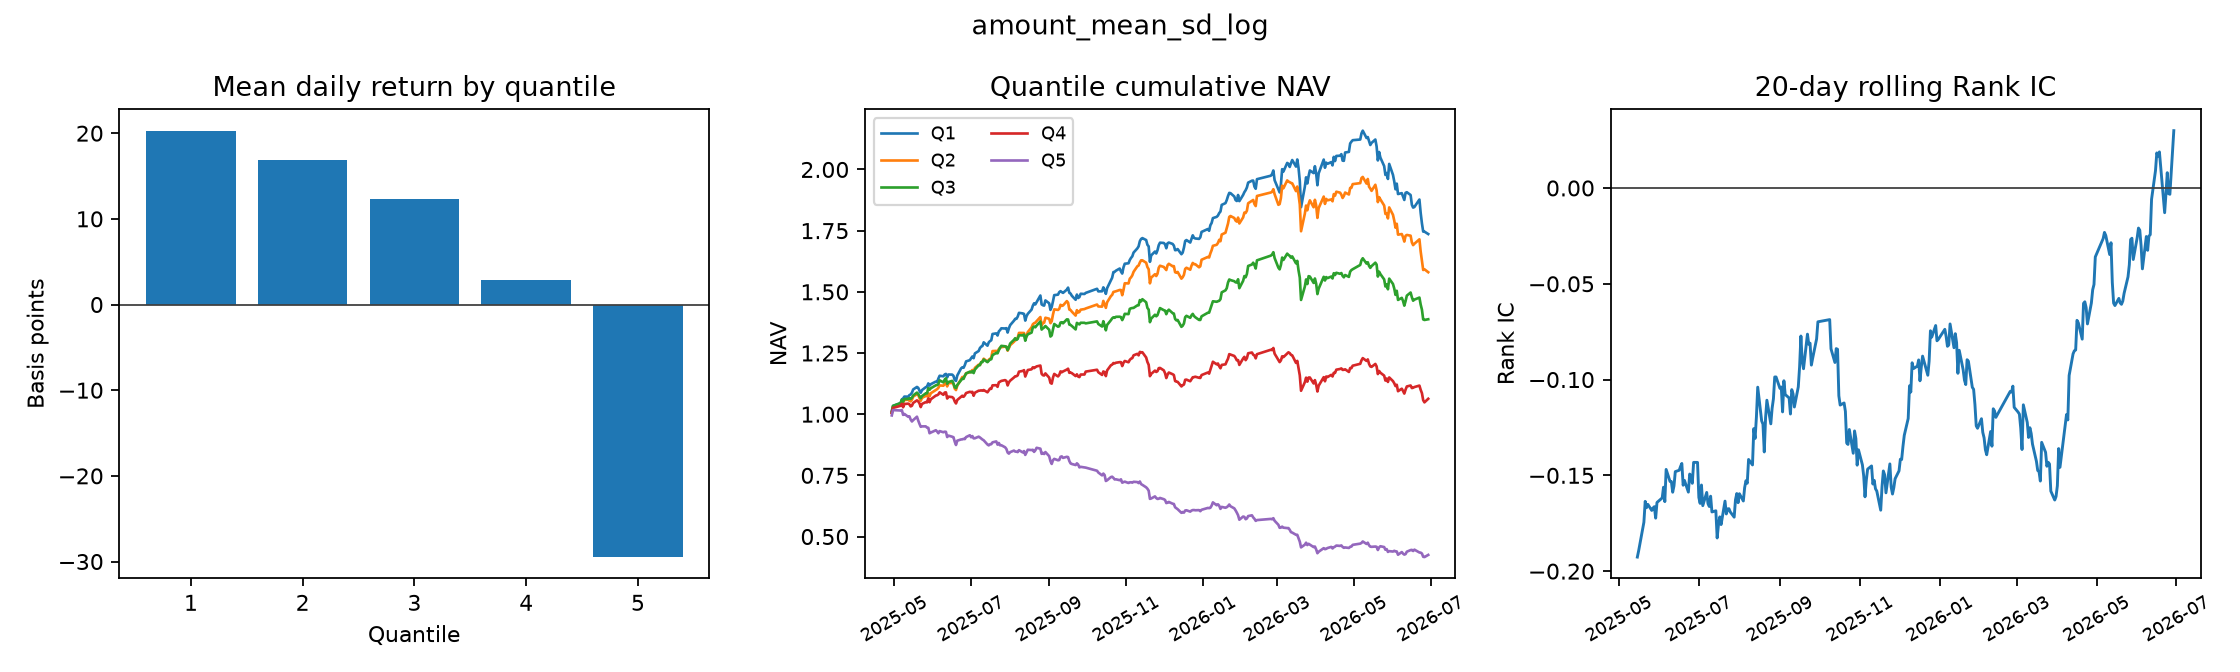
\includegraphics[width=0.96\textwidth]{qr_factor_amount.png}
\caption{成交额多窗口均值离散度因子诊断。负 Rank IC 和下降的分组收益说明该因子应反向使用。}
\end{figure}

\begin{figure}[H]\centering
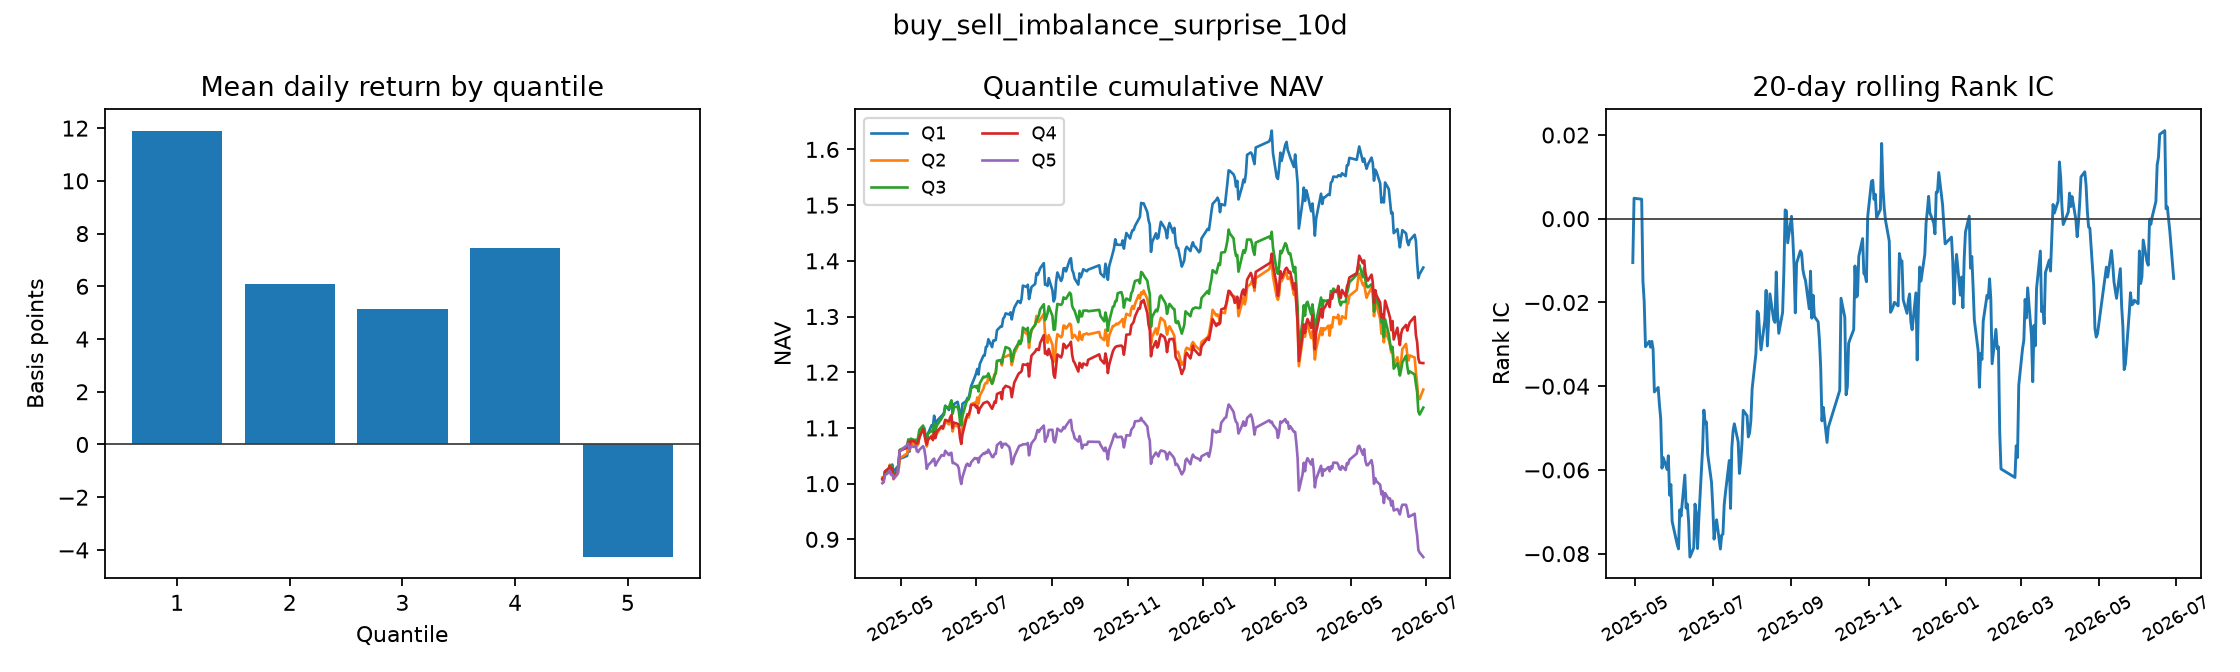
\includegraphics[width=0.96\textwidth]{qr_factor_imbalance.png}
\caption{主动买卖不平衡因子诊断。其 Rank IC 接近零，单因子预测力较弱，因此不应单独承担组合方向。}
\end{figure}

\begin{figure}[H]\centering
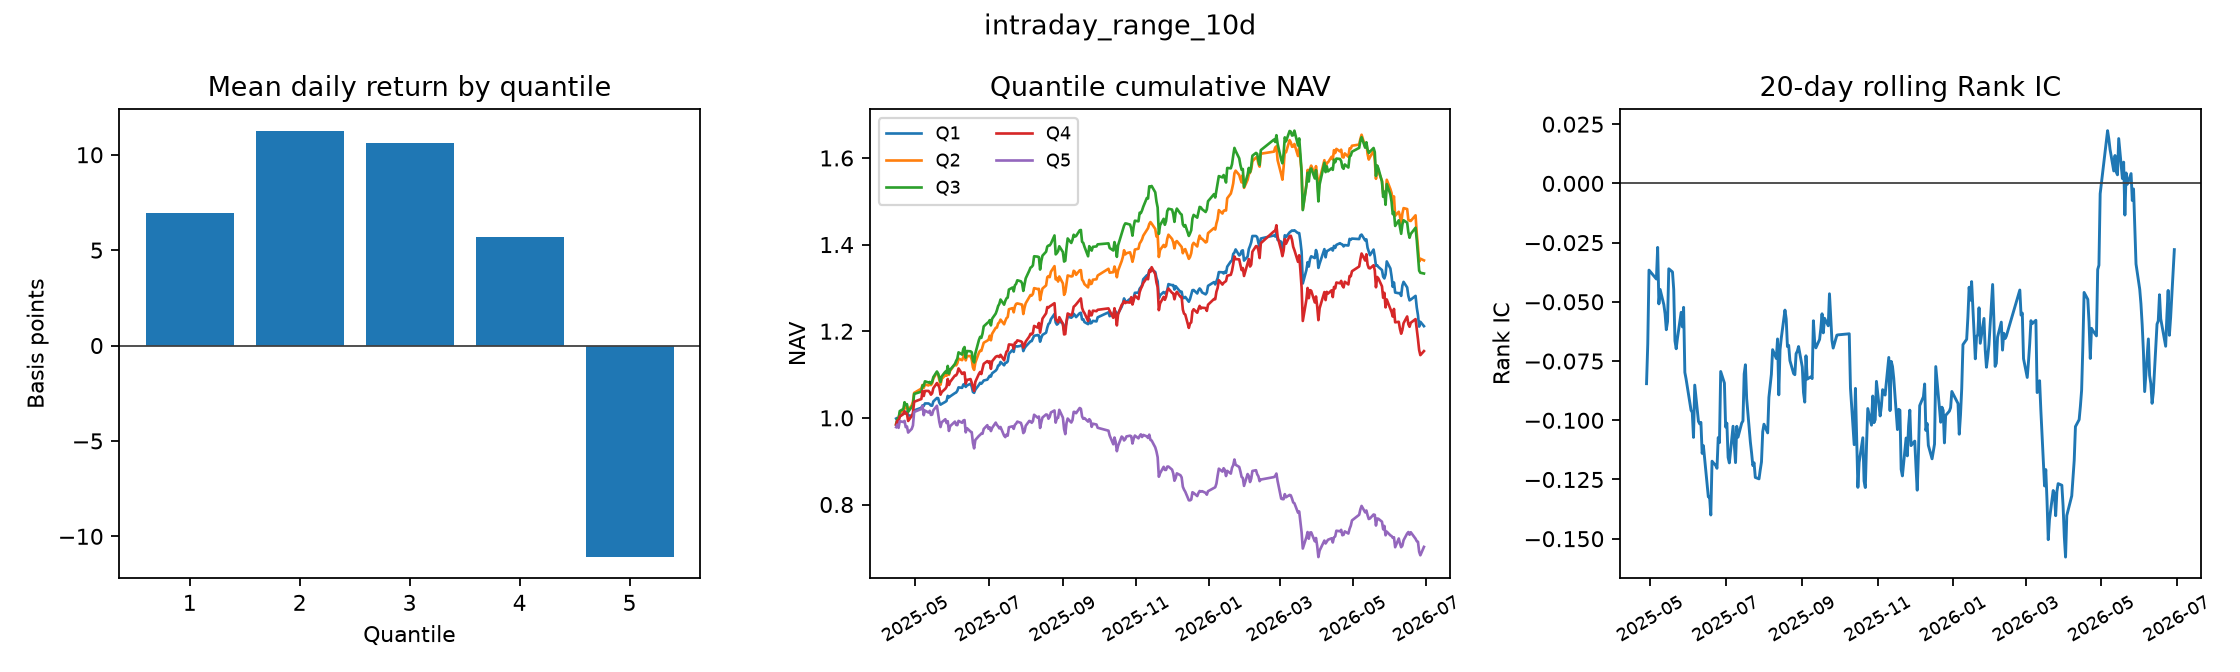
\includegraphics[width=0.96\textwidth]{qr_factor_range.png}
\caption{10日日内振幅因子诊断。高振幅组未来收益较弱，表现为稳定的负向因子。}
\end{figure}

\begin{figure}[H]\centering
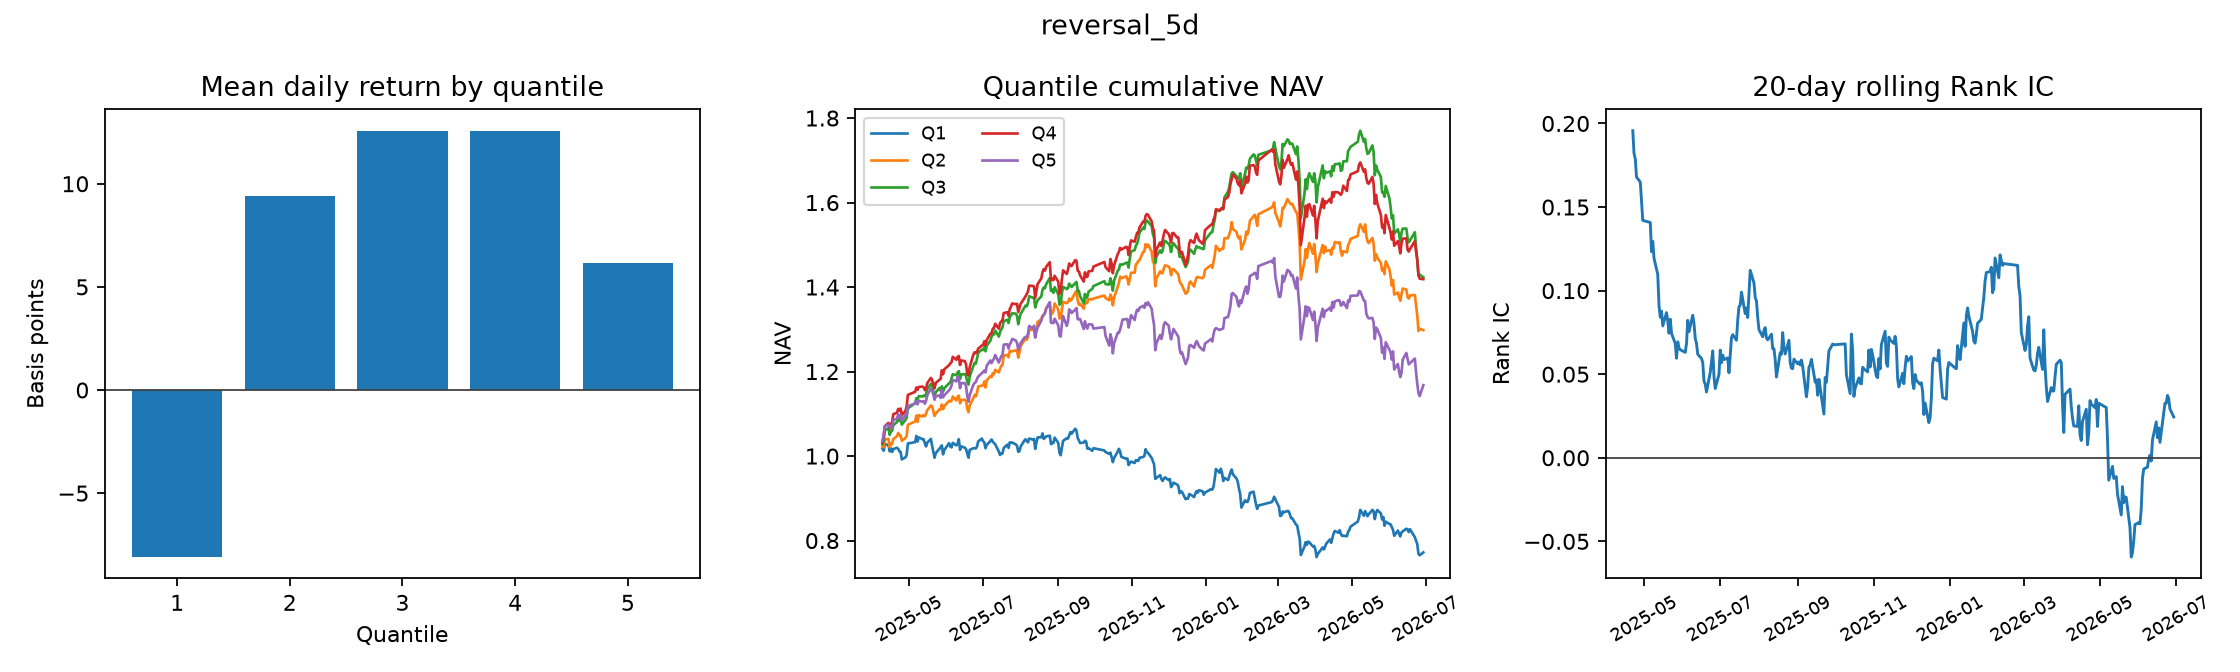
\includegraphics[width=0.96\textwidth]{qr_factor_reversal.png}
\caption{5 日反转因子诊断。正 Rank IC 与正多空收益表明近期弱势股票随后存在一定反弹。}
\end{figure}

\begin{figure}[H]\centering
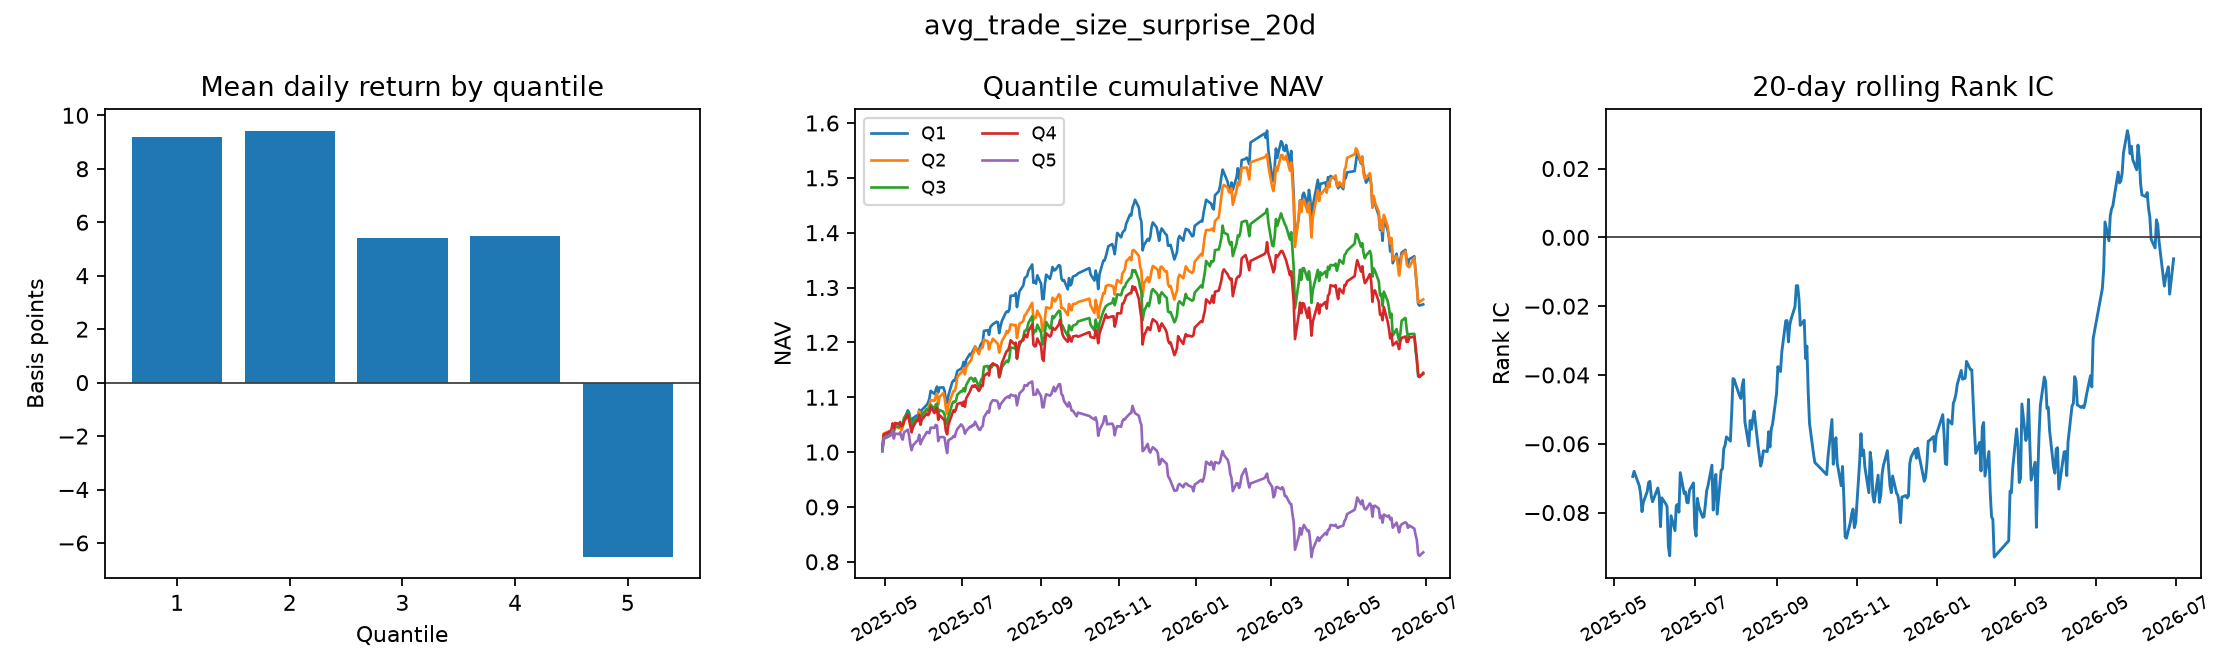
\includegraphics[width=0.96\textwidth]{qr_factor_trade_size.png}
\caption{20 日单笔成交规模异常因子诊断。异常放大的平均单笔成交规模与下一日收益呈负相关。}
\end{figure}

\begin{figure}[H]\centering
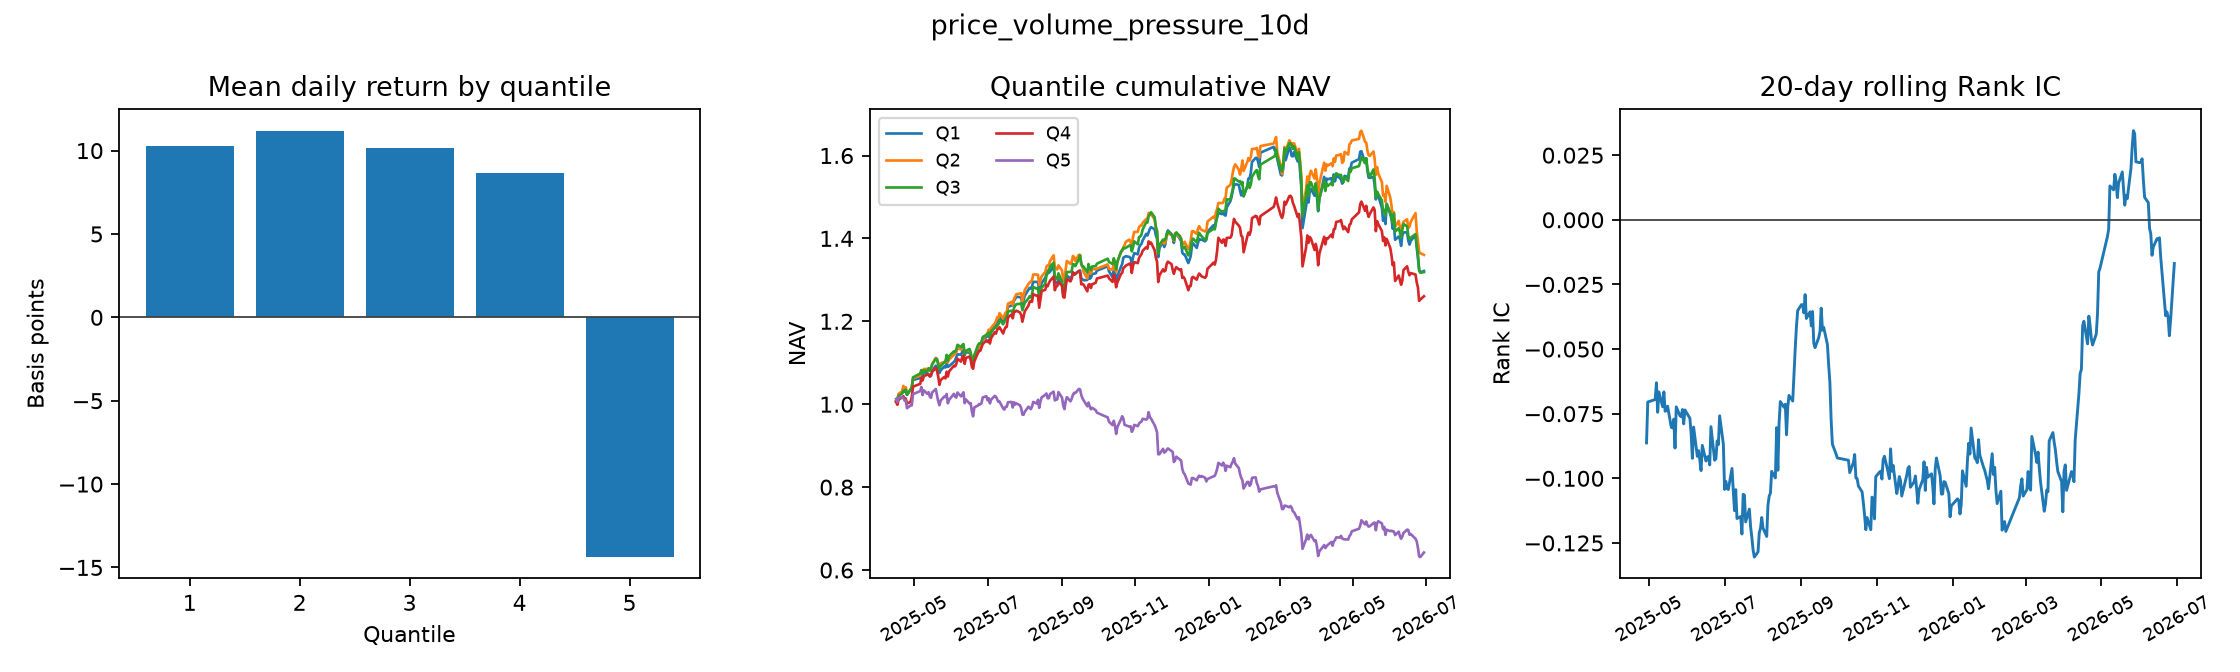
\includegraphics[width=0.96\textwidth]{qr_factor_price_volume.png}
\caption{10 日价量压力因子诊断。该因子呈负向预测，显示近期价量同向压力可能伴随后续修正。}
\end{figure}

\begin{figure}[H]\centering
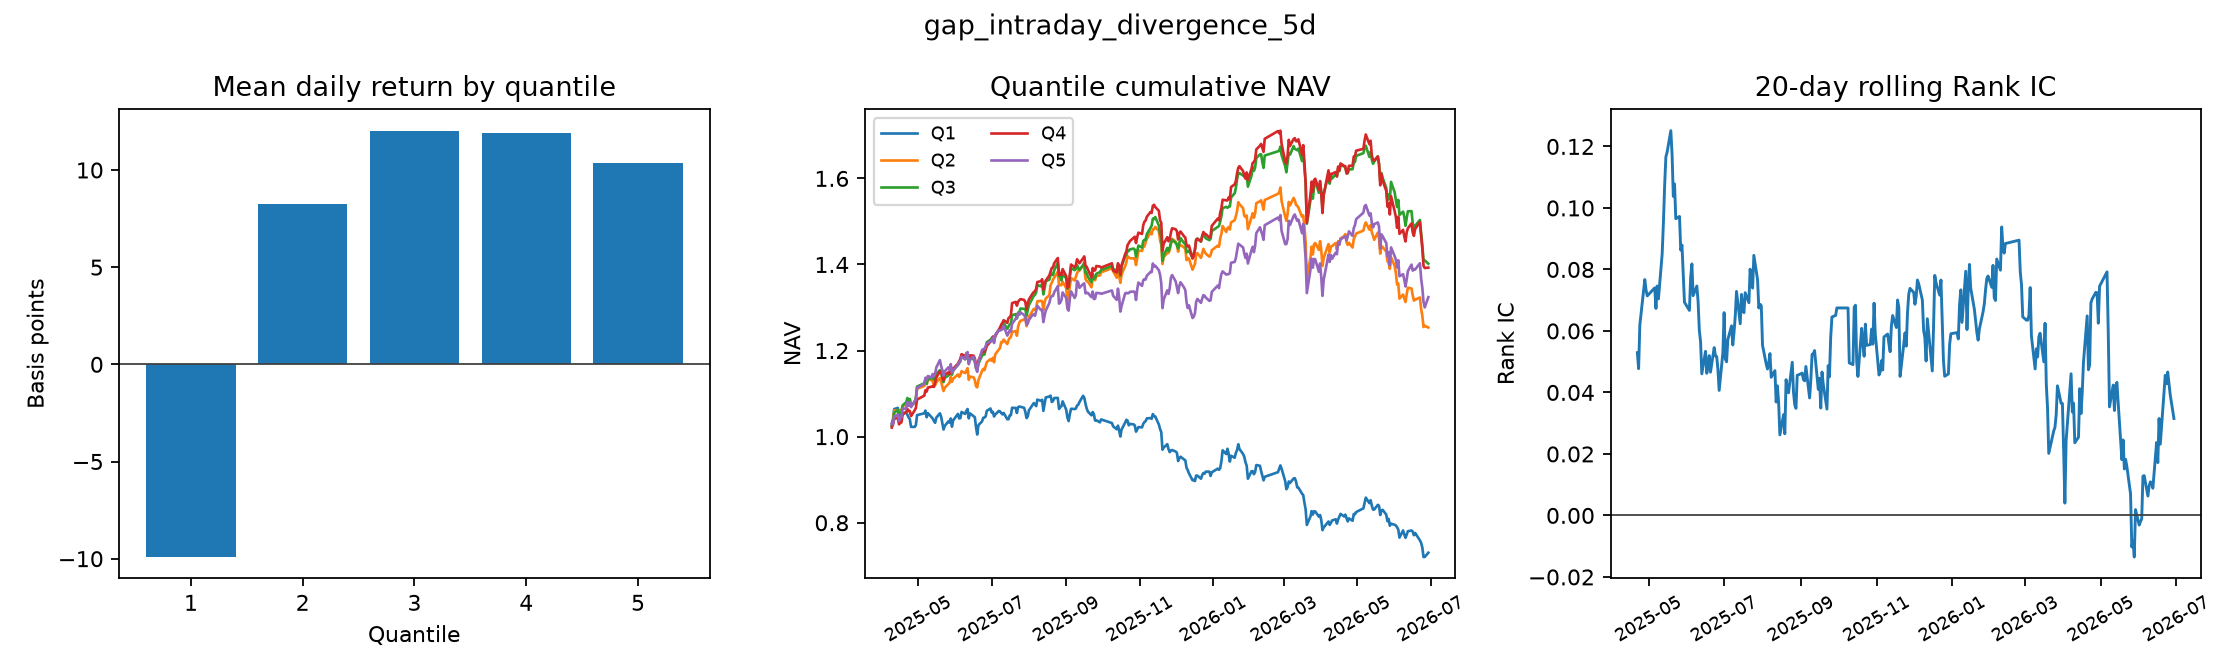
\includegraphics[width=0.96\textwidth]{qr_factor_gap_intraday.png}
\caption{5 日隔夜--日内收益背离因子诊断。其 Q5--Q1 累计收益为 80.41\%，是新增因子中表现最强的一项。}
\end{figure}

\section{相关性与多空净值}

因子相关性用于识别重复信息。18 因子中，特质波动率与普通已实现波动率的相关系数约为 -0.959，说明两者包含大量重复风险信息；因此新增风险因子不能仅凭单因子 IC 直接叠加进正式信号。完整组合在留出期回撤恶化，最终版本保留原 15 因子排序，只采用独立的组合波动率目标。

\begin{figure}[H]\centering
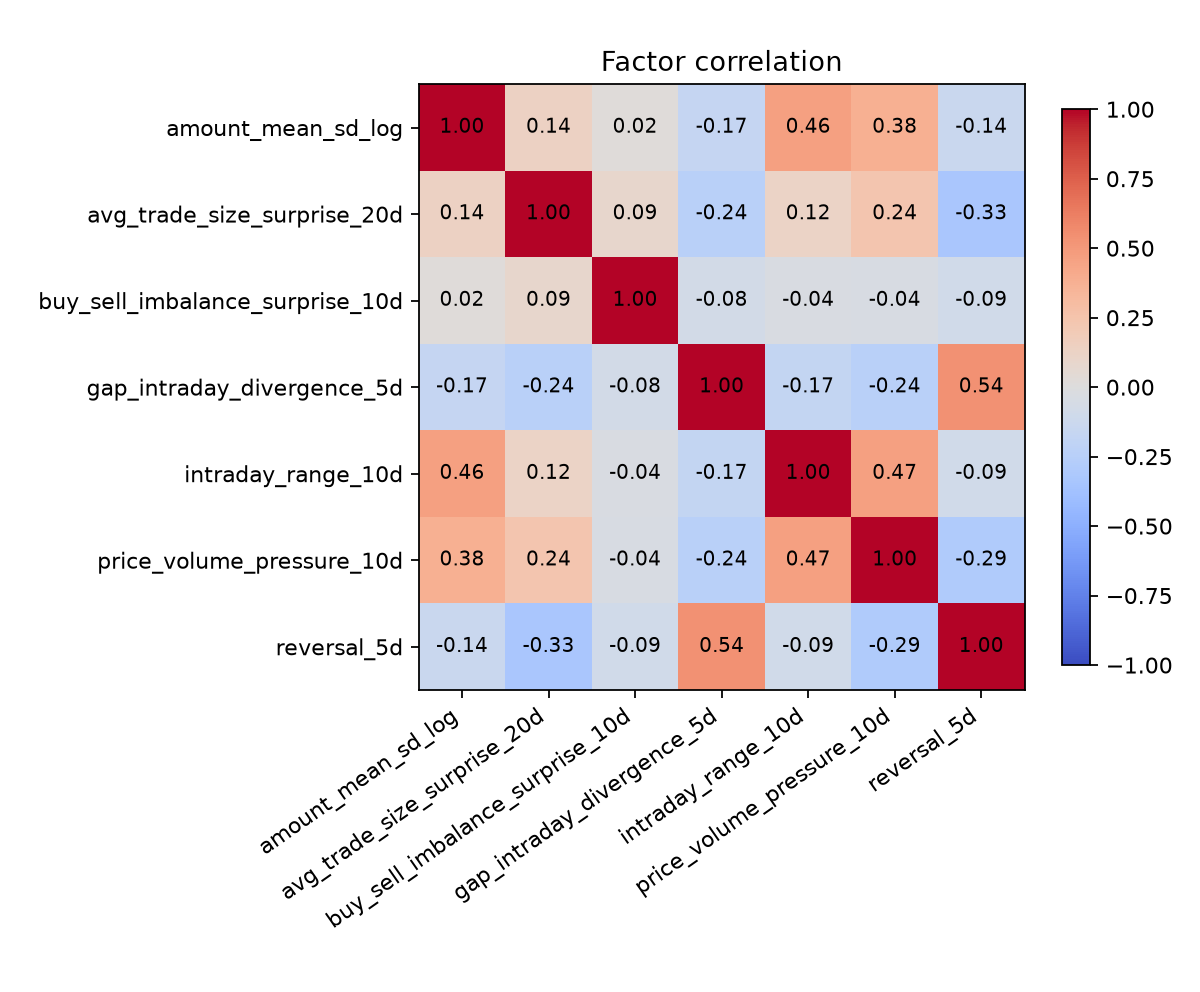
\includegraphics[width=0.86\textwidth]{qr_factor_corr.png}
\caption{18 因子横截面相关系数热力图。新增风险因子与传统波动率因子存在明显重叠。}
\end{figure}

\begin{figure}[H]\centering
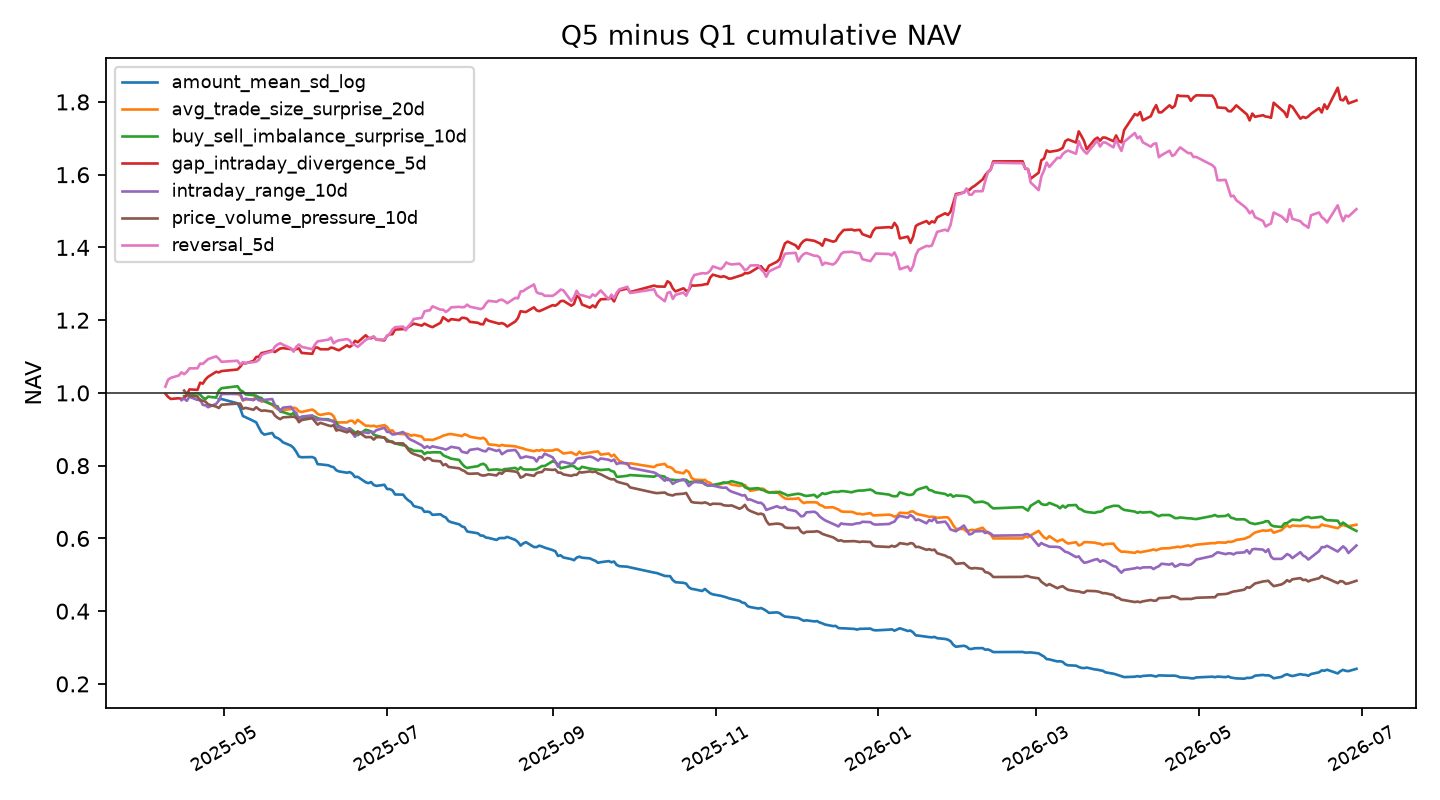
\includegraphics[width=0.94\textwidth]{qr_factor_ls_nav.png}
\caption{18 因子 Q5--Q1 多空累计净值。正负方向不同的因子在组合前按 historical IC 调整方向。}
\end{figure}

\chapter{组合构建与无前视回测}

\section{Historical IC 加权形成综合信号}

因子 $k$ 在交易日 $t$ 的方向和权重只使用截至 $t-1$ 的 20 日 historical IC：
\begin{equation}
\bar{IC}_{k,t}=\frac{1}{20}\sum_{s=t-20}^{t-1}IC_{k,s},\qquad
w_{k,t}=\frac{\bar{IC}_{k,t}}{\sum_j |\bar{IC}_{j,t}|}.
\end{equation}
综合得分为
\begin{equation}
Score_{i,t}=\sum_k w_{k,t}z_{i,k,t}.
\end{equation}
这里不能使用 $IC_{k,t}=\mathrm{corr}(F_{k,t},R_{t+1})$ 直接决定 $t$ 日交易，因为 $R_{t+1}$ 在下单时尚未发生。

\section{风险候选权重与最终采用规则}

为降低风险，研究额外测试了 60 日 EWMA ICIR 权重。先用截至 $t-1$ 的 IC 序列计算指数加权均值与标准差：
\begin{equation}
q_{k,t}=\frac{\mathrm{EWMA}_{60}(IC_{k,s},s\le t-1)}
{\mathrm{EWSD}_{60}(IC_{k,s},s\le t-1)},\qquad
w^{risk}_{k,t}=\mathrm{clip}\!\left(\frac{q_{k,t}}{\sum_j|q_{j,t}|},-0.25,0.25\right).
\end{equation}
同时测试正向综合得分乘逆 20 日波动率的个股权重：
\begin{equation}
\tilde w_{i,t}\propto \frac{\mathrm{PositiveScore}_{i,t}}{\widehat\sigma^{20}_{i,t}},
\qquad \tilde w_{i,t}\le 4\%.
\end{equation}
若股票因停牌或涨跌停无法交易，其冻结仓位可暂时超过 4\%。拆解结果显示，上述两项与新增风险因子一起替换原信号时，留出期最大回撤由 -10.90\% 恶化至 -18.25\%，因此不予采用。

最终采用的规则仅改变组合总敞口。令 $r^{p}_{s}$ 为策略在当日之前已经实现的毛收益，使用最近 20 日年化波动率估计：
\begin{equation}
\widehat\sigma^{p}_{t-1}=\mathrm{SD}(r^{p}_{t-20},\ldots,r^{p}_{t-1})\sqrt{252},
\qquad
L_t=\mathrm{clip}\!\left(\frac{15\%}{\widehat\sigma^{p}_{t-1}},0.5,1.0\right).
\end{equation}
历史不足 20 日时使用 $L_t=1$。该规则只使用当前交易日之前的组合收益，因而不存在前视信息。

\section{换手控制与持仓规则}

持仓 30 只，调仓频率为每 5 个交易日，已持有股票只要仍位于综合排名前 60 就继续保留，再从最新排名中补足 30 只。缓冲区使排名第 30 与第 31 的微小变化不再自动触发交易。

\begin{figure}[H]\centering
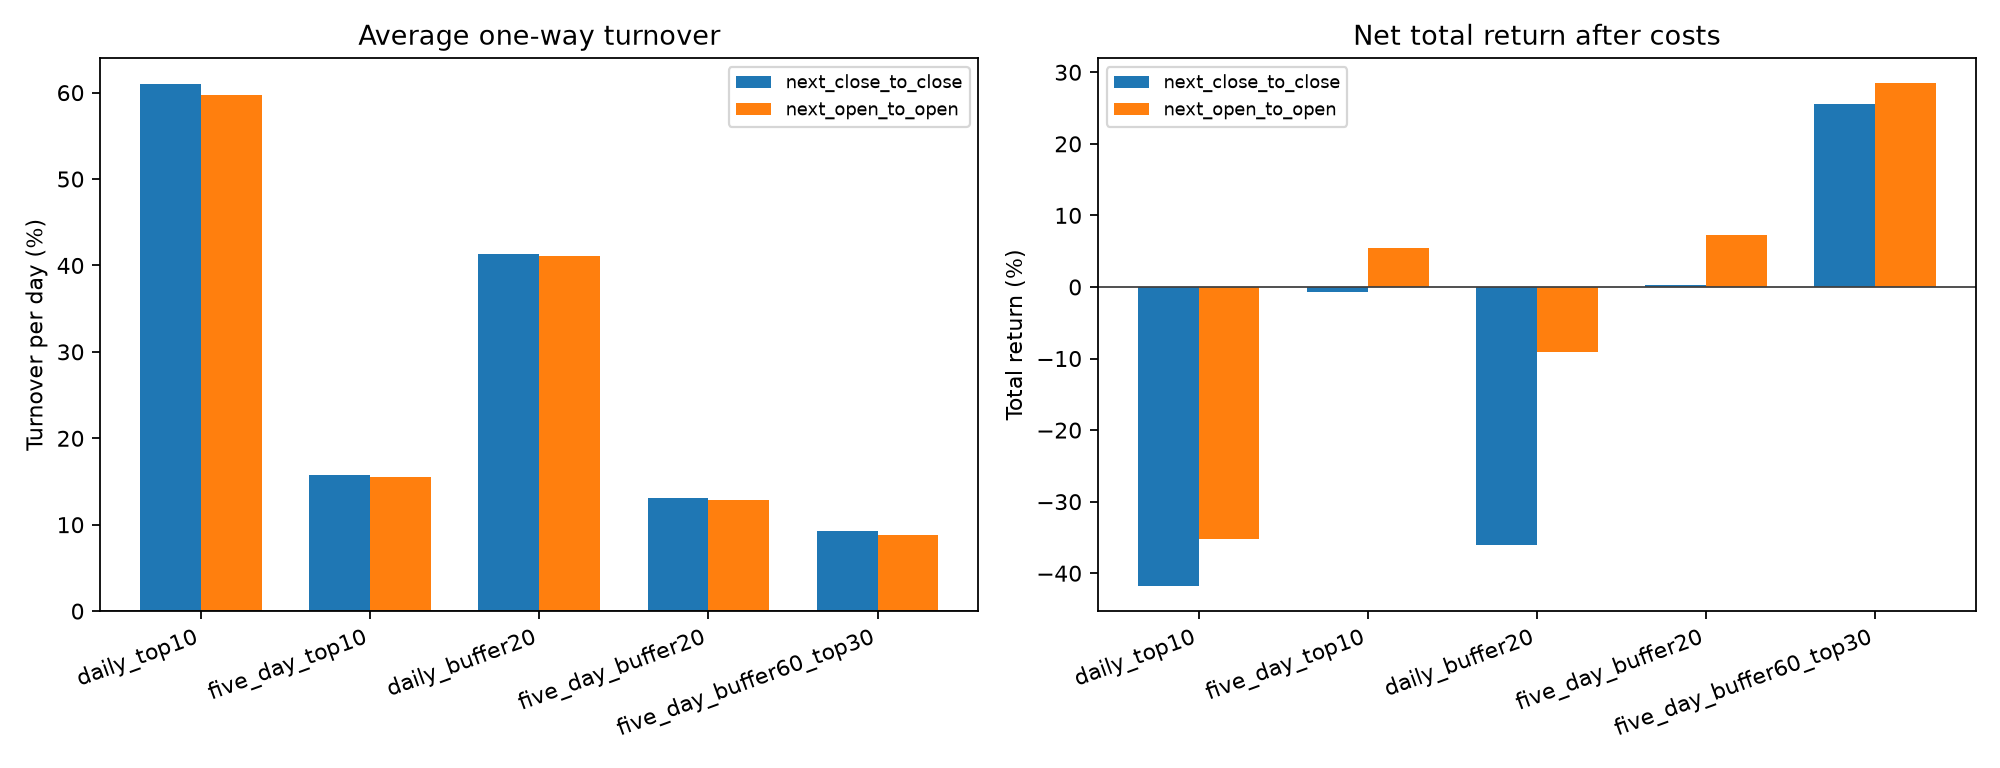
\includegraphics[width=0.96\textwidth]{qr_turnover_comparison.png}
\caption{不同换手控制政策比较。最新次日开盘基线的日均单边换手率为 8.81\%。}
\end{figure}

\section{成交时点、限制与交易成本}

信号在 $t$ 日形成，只能在 $t+1$ 日开盘或收盘成交，随后持有到下一对应价格时点。成交量或成交额为零视为停牌；一字涨停不能买入，一字跌停不能卖出；无法卖出的股票继续保留。

\noindent 成本由三部分组成：卖出金额的 5 个基点手续费；买卖双方各 5 个基点基础滑点；以及订单金额占当日成交额比例驱动的平方根冲击：
\begin{equation}
c^{impact}_{i,t}=\min\left(c_{max},\eta\sqrt{\frac{Q_{i,t}}{ADV_{i,t}}}\right).
\end{equation}
其中 $Q$ 为订单金额，$ADV$ 为日成交额，$\eta$ 为冲击系数。该设计使低流动性股票和大额订单承担更高成本。

\chapter{风险收益结果与稳健性检验}

\section{绩效指标定义}

累计收益为 $\prod_t(1+r_t)-1$；年化收益为 $(1+R)^{252/T}-1$；年化波动率为 $\sigma(r)\sqrt{252}$；最大回撤为净值相对历史峰值的最小跌幅；夏普率为年化平均超额于无风险利率后的收益除以年化波动；信息比率为主动收益均值除以跟踪误差并年化。等权基准使用入场日可以买入股票的当日等权收益。

\begin{table}[H]
\centering
\caption{最终策略完整样本风险收益}
\begin{tabular}{lrr}
\toprule
指标 & 次日收盘 & 次日开盘 \\
\midrule
成本前累计收益 & 37.97\% & 38.33\% \\
成本后累计收益 & 27.52\% & 28.30\% \\
年化收益 & 24.96\% & 25.66\% \\
年化超额收益 & 20.65\% & 23.02\% \\
年化波动率 & 18.84\% & 18.50\% \\
最大回撤 & -11.93\% & -10.90\% \\
夏普率 & 1.277 & 1.327 \\
信息比率 & 1.880 & 1.838 \\
日均单边换手 & 9.22\% & 8.81\% \\
总交易成本 & 951,129 & 911,060 \\
\bottomrule
\end{tabular}
\end{table}

\begin{figure}[H]\centering
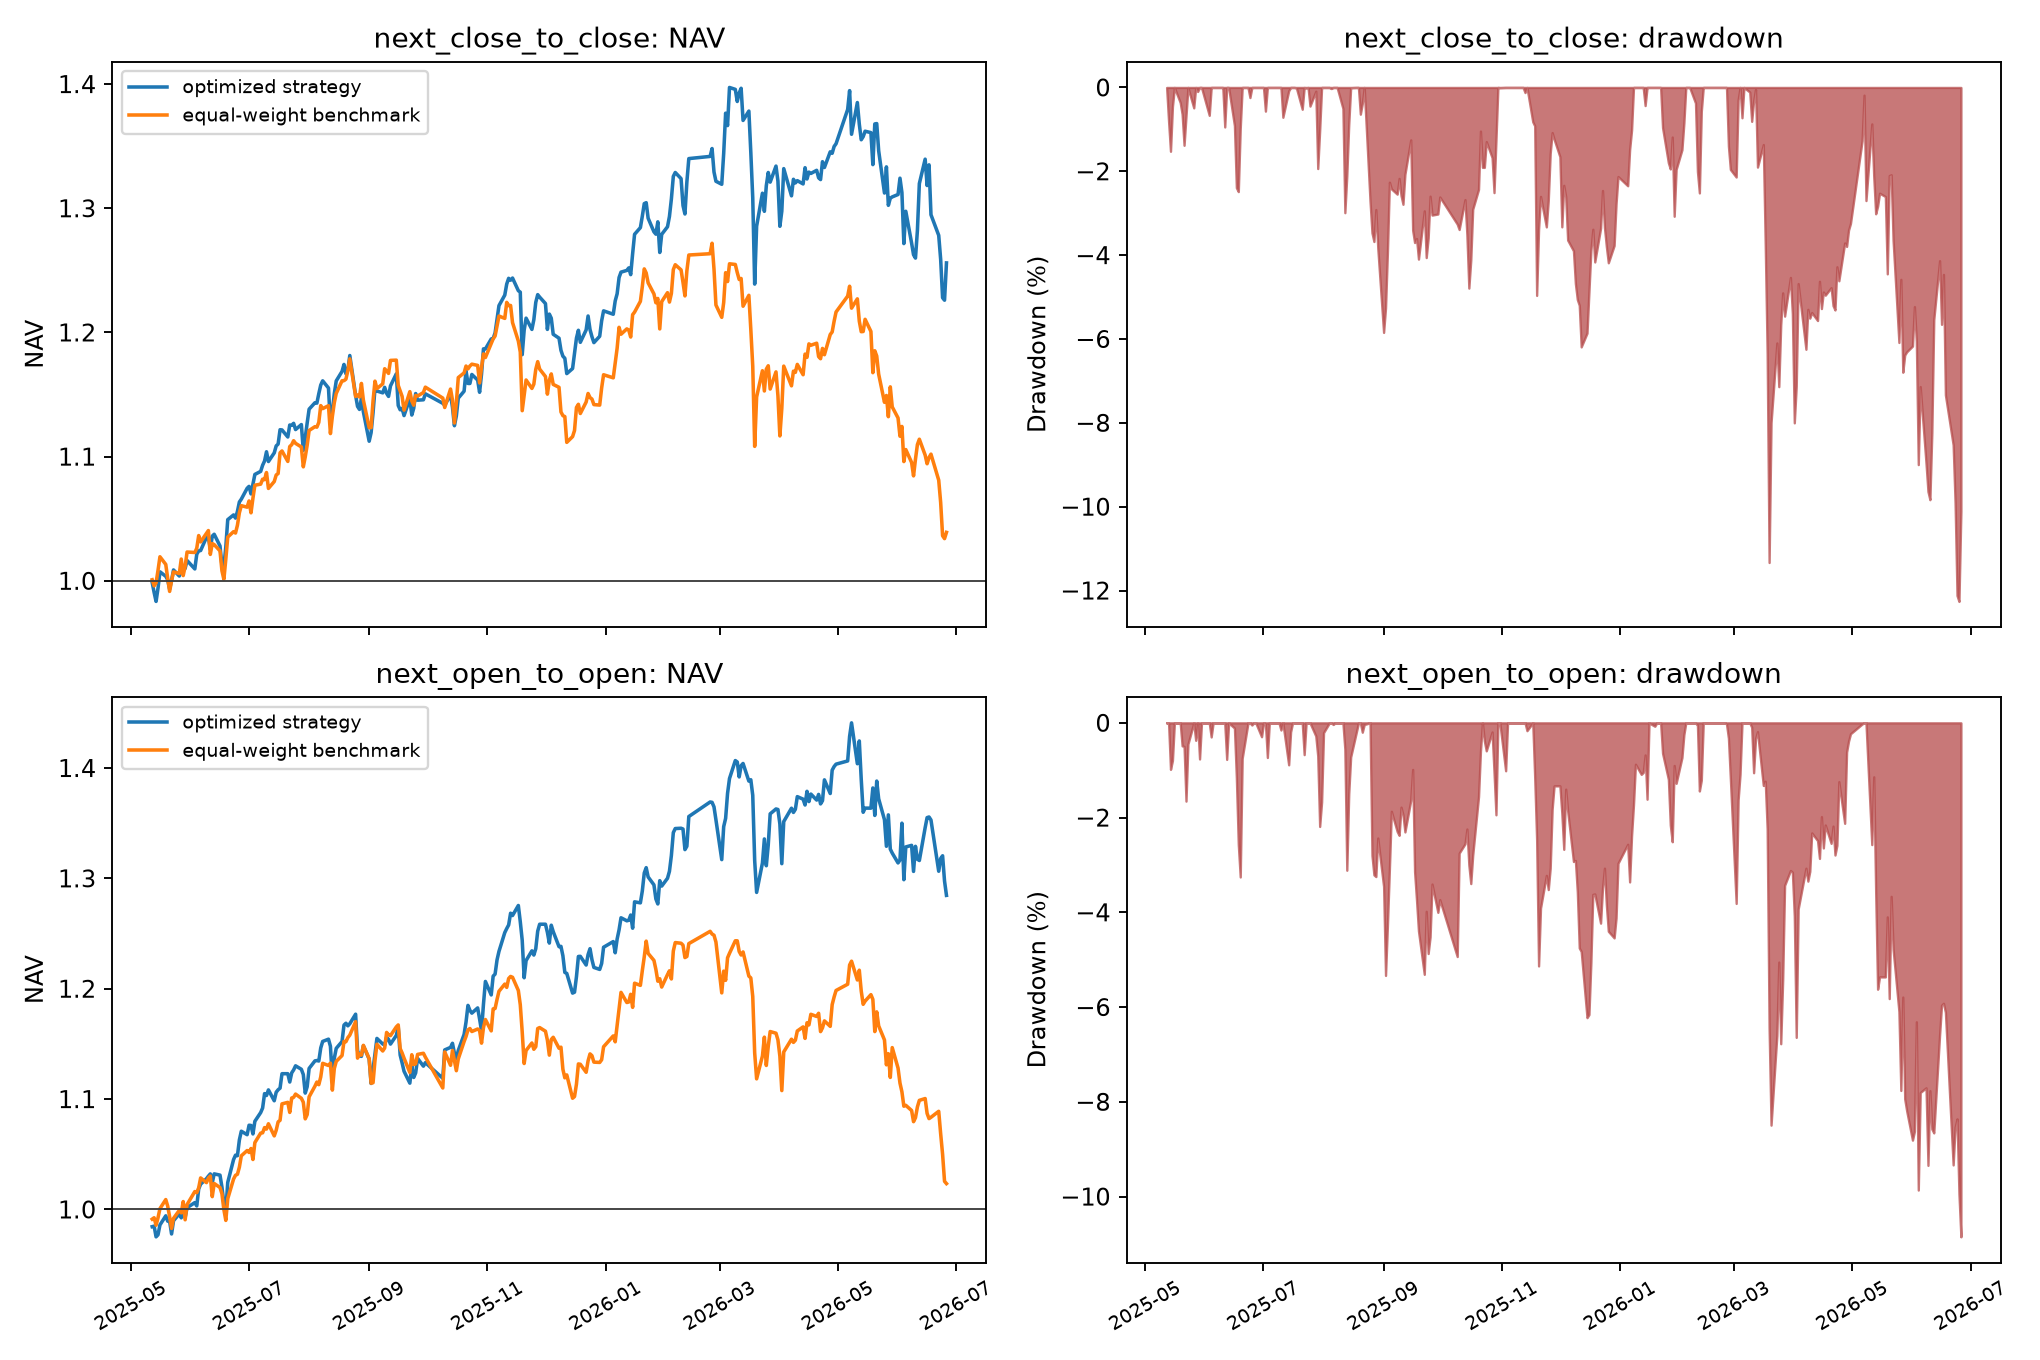
\includegraphics[width=0.98\textwidth]{qr_nav_drawdown.png}
\caption{正式因子策略净值、等权基准与回撤。次日开盘结果在收益和回撤两方面优于次日收盘。}
\end{figure}

\begin{figure}[H]\centering
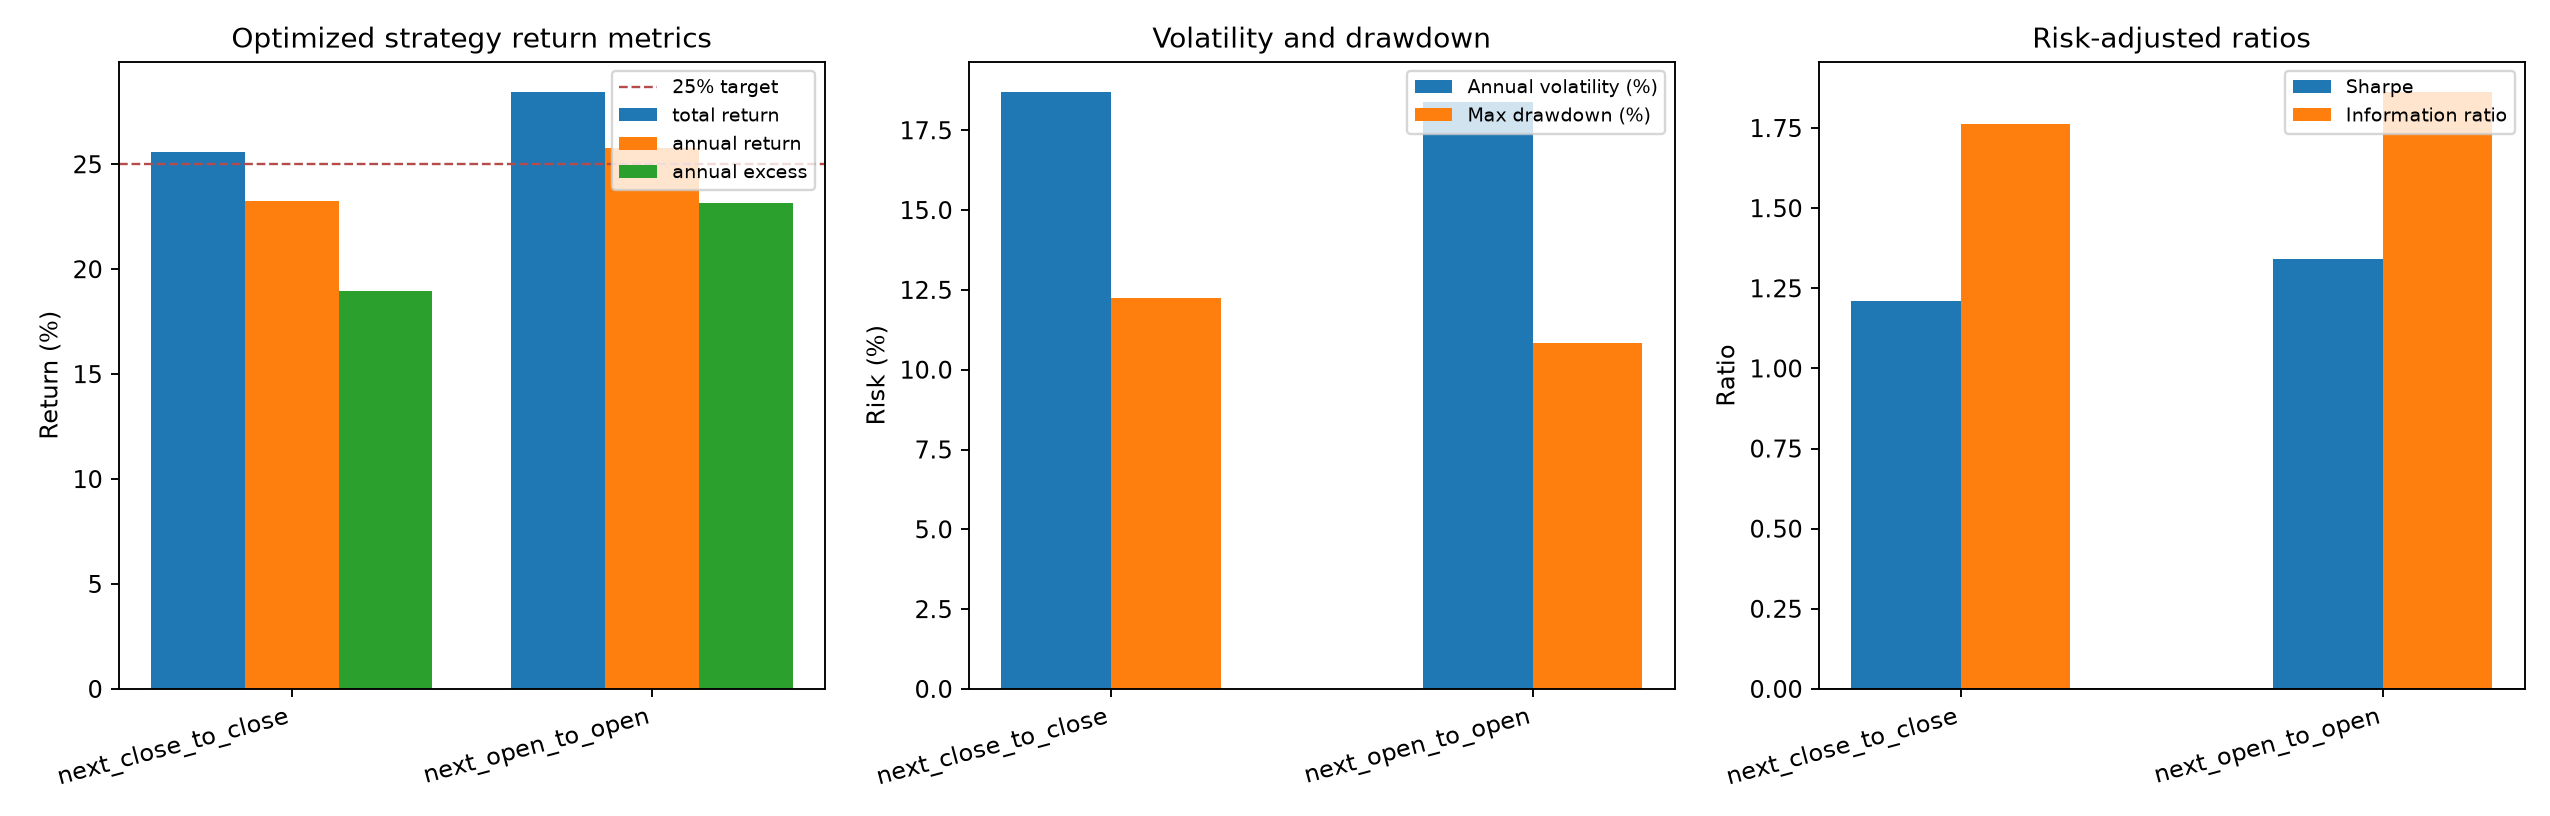
\includegraphics[width=0.96\textwidth]{qr_risk_metrics.png}
\caption{收益、波动、回撤、夏普率、信息比率和换手率的并列比较。}
\end{figure}

\section{15\% 波动率目标与风险拆解}

表中将原 15 因子 1 倍基线、固定 1.24 倍敞口和最终采用的 15\% 波动率目标进行直接比较。动态目标在完整样本中牺牲约 0.71 个百分点的年化收益，相对 1 倍基线把波动率从 18.50\% 降至 16.33\%，最大回撤从 -10.90\% 改善至 -9.58\%；相对固定 1.24 倍版本的风险改善更明显。

\begin{table}[H]
\centering
\small
\caption{次日开盘风险预算对比}
\begin{tabular}{llrrrr}
\toprule
样本 & 版本 & 累计收益 & 年化收益 & 年化波动 & 最大回撤 \\
\midrule
完整样本 & 原信号 1 倍 & 28.30\% & 25.66\% & 18.50\% & -10.90\% \\
完整样本 & 固定 1.24 倍 & 33.30\% & 30.13\% & 22.94\% & -13.60\% \\
完整样本 & 15\% 波动率目标 & 27.52\% & 24.95\% & 16.33\% & -9.58\% \\
\midrule
后 20\% 留出期 & 原信号 1 倍 & -5.16\% & -21.54\% & 23.06\% & -10.90\% \\
后 20\% 留出期 & 固定 1.24 倍 & -6.79\% & -27.54\% & 28.58\% & -13.60\% \\
后 20\% 留出期 & 15\% 波动率目标 & -4.10\% & -17.44\% & 18.35\% & -9.58\% \\
\bottomrule
\end{tabular}
\end{table}

\begin{figure}[H]\centering
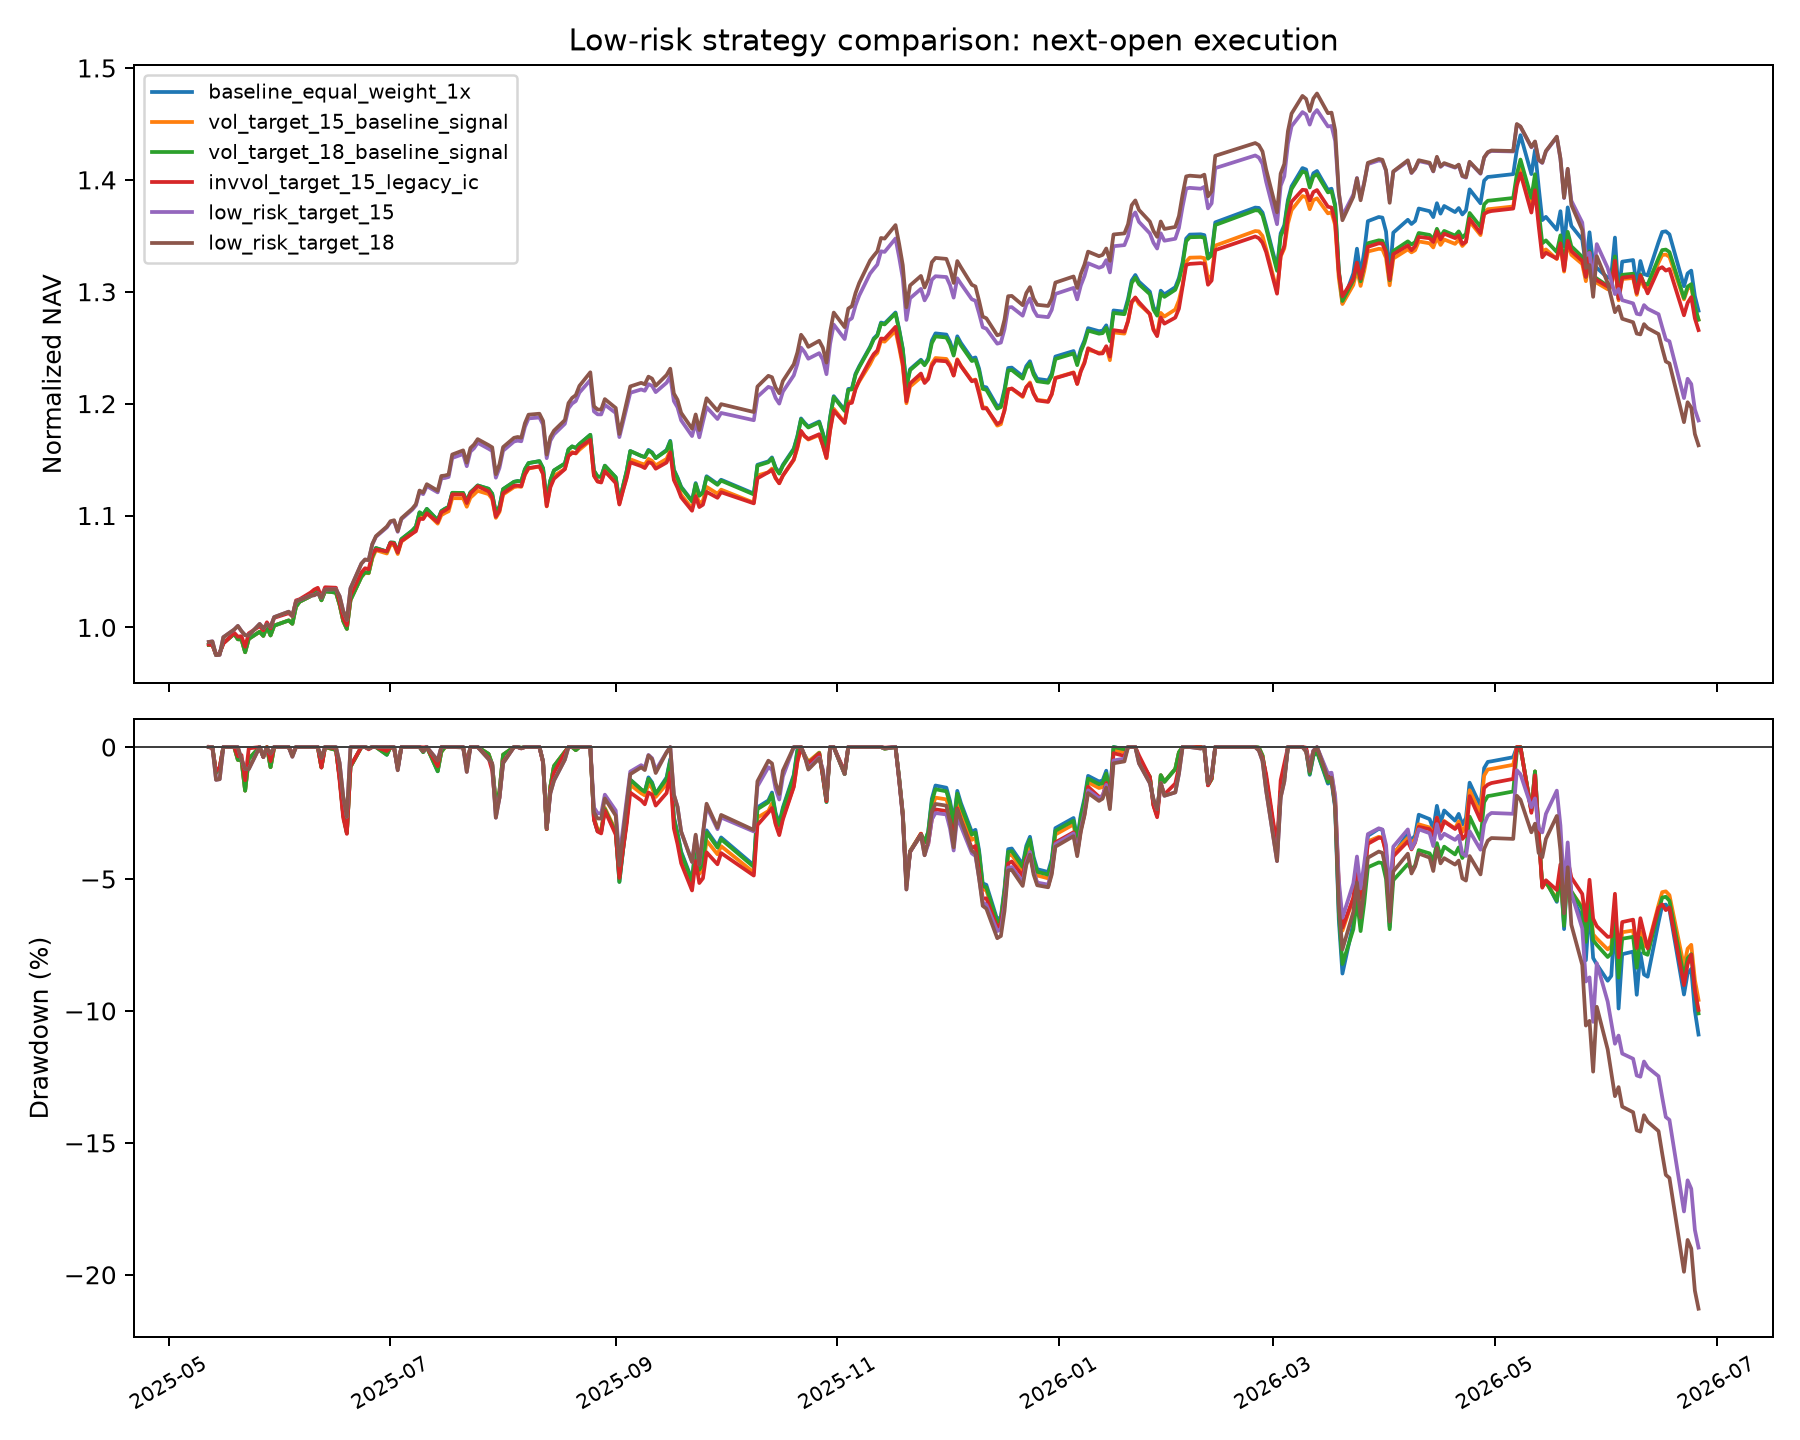
\includegraphics[width=0.98\textwidth]{qr_low_risk_nav_drawdown.png}
\caption{风险版本净值与回撤拆解。完整替换因子与 IC 权重的版本虽然降低波动，但留出期回撤恶化；最终采用的是保留原信号的 15\% 波动率目标。}
\end{figure}

\section{研究期与留出期}

为区分研究选择效应与时间外推能力，样本按时间切分为前 80\% 研究期和后 20\% 留出期。最终 15\% 波动率目标策略在研究期累计收益 32.97\%，在留出期为 -4.10\%；同期留出期等权基准为 -10.44\%，累计主动收益为 7.08\%。这说明动态敞口在下跌环境中改善了绝对风险和相对收益，但尚未证明稳定的正绝对收益。

\begin{figure}[H]\centering
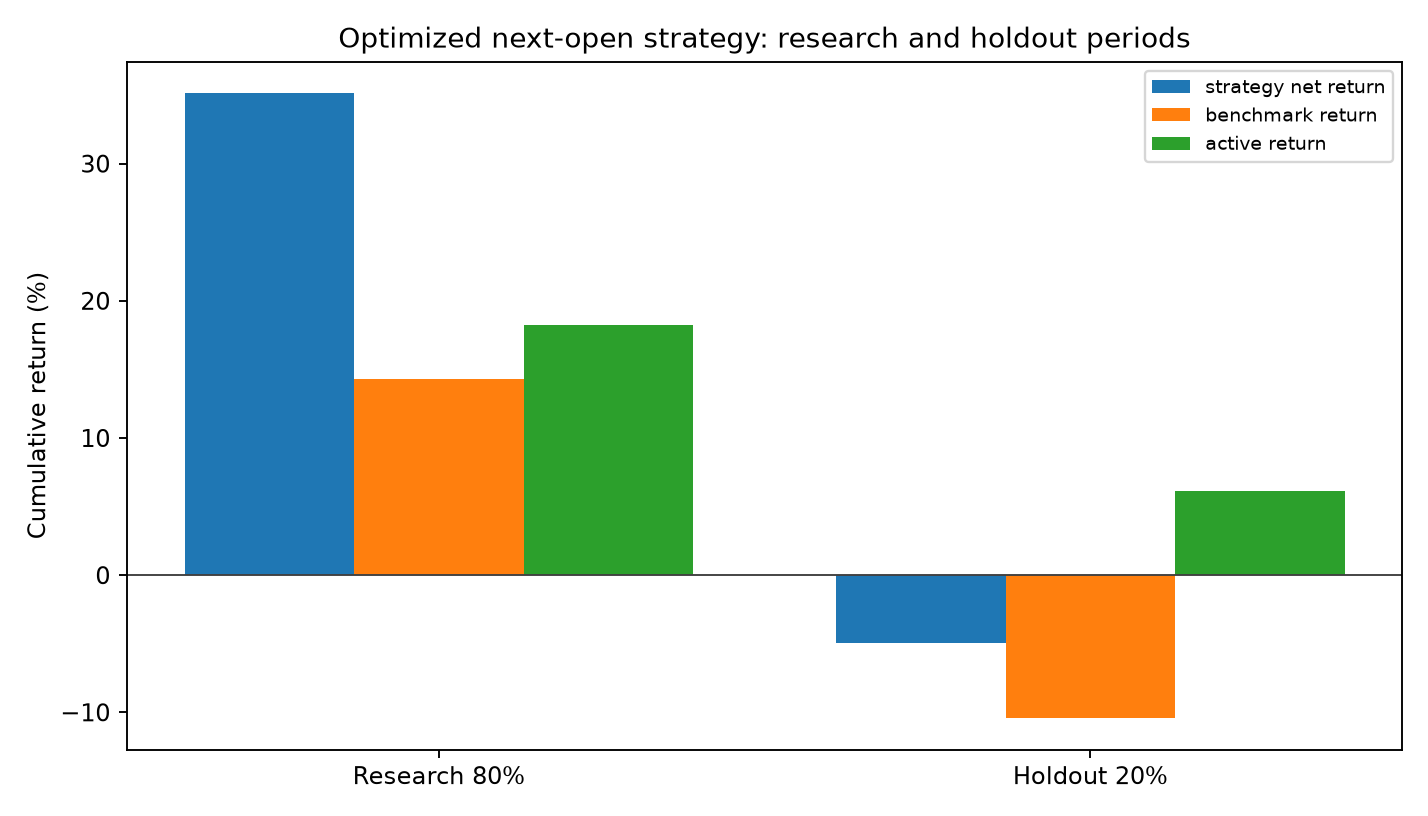
\includegraphics[width=0.96\textwidth]{qr_period_split.png}
\caption{原 1 倍基线的完整样本、前 80\% 研究期与后 20\% 留出期比较；最终风险目标的分阶段数据另见表~\ref{tab:period_backtest}。}
\end{figure}

\clearpage
\subsubsection{样本期划分与定义}

本研究将全部数据按时间划分为前 80\% 研究期和后 20\% 时间留出检查。研究期用于因子探索、模型拟合、参数选择和验证；后 20\% 原本作为留出期，但本轮已经用于比较风险版本和确定最终规则，因此只能称为准样本外检查，不能继续称为独立样本外证据。“样本外”应仅用于完全未参与当前模型拟合及参数选择的数据。全样本结果同时包含研究期和后 20\% 区间，也不视为独立样本外证据。


\begin{table}[H]
\centering
\caption{样本期统一定义}
\small

\begin{tabularx}{\textwidth}{
    >{\raggedright\arraybackslash}p{3.2cm}
    >{\raggedright\arraybackslash}X
    >{\raggedright\arraybackslash}X
}
\toprule
术语 & 定义 & 用途 \\
\midrule

全样本（Full Sample）
& 报告覆盖的全部日期，包括研究期和独立留出期
& 展示总体净值、收益、回撤和交易成本 \\

研究期（Research Period）
& 用于因子探索、策略设计、模型拟合和参数选择的区间
& 确定因子、持仓数量、调仓频率、缓冲区和成本参数 \\

验证期（Validation Period）
& 研究期内部用于模型选择、超参数选择、阈值选择和早停的区间
& 比较候选方案并确定最终配置 \\

后 20\% 留出检查（Holdout Check）
& 按时间后移的数据，但本轮已用于风险版本比较
& 准样本外稳健性检查，不作为严格 OOS 证明 \\

样本外（Out-of-Sample）
& 某次预测或回测使用了未参与当前模型拟合及参数选择的数据
& 描述 Walk-forward 测试窗口或独立留出期结果 \\

\bottomrule
\end{tabularx}
\end{table}

\subsubsection{分阶段回测结果}

为区分研究选择效应与时间外推能力，
分别报告研究期、后 20\% 留出检查及全样本的回测结果。

\begin{table}[H]
\centering
\small
\begin{threeparttable}

\caption{分阶段回测结果}
\label{tab:period_backtest}

\renewcommand{\arraystretch}{1.5}

\begin{tabularx}{\textwidth}{
    >{\raggedright\arraybackslash}p{2.7cm}
    >{\raggedright\arraybackslash}X
    >{\centering\arraybackslash}p{2.0cm}
    >{\centering\arraybackslash}p{2.2cm}
    >{\centering\arraybackslash}p{2.0cm}
    >{\raggedright\arraybackslash}p{2.3cm}
}
\toprule
\textbf{区间}
& \textbf{数据用途}
& \textbf{策略累计收益}
& \textbf{等权基准累计收益}
& \textbf{累计主动收益}
& \textbf{结果性质} \\
\midrule

研究期（前80\%）
& 因子研究、参数选择和策略开发
& 32.97\%
& 14.27\%
& 16.36\%
& 研究期结果 \\

\midrule

后 20\% 留出检查
& 风险版本比较与稳健性检查
& -4.10\%
& -10.44\%
& 7.08\%
& 准样本外检查\tnote{*} \\

\midrule

全样本
& 总体净值和风险展示
& 27.52\%
& 2.34\%
& 24.60\%
& 全样本回测结果 \\

\bottomrule
\end{tabularx}

\begin{tablenotes}[flushleft]
\footnotesize
\item[*]
后 20\% 区间已参与本轮风险版本比较，因此不再标记为严格独立样本外。
主动收益按照策略净值相对于基准净值计算，不能直接用两个累计收益率相减。
\end{tablenotes}

\end{threeparttable}
\end{table}

\noindent 最终 15\% 波动率目标策略在研究期累计收益为 32.97\%，在后 20\% 区间的绝对收益为 -4.10\%。同期等权基准累计收益为 -10.44\%，策略在下跌环境中表现出相对抗跌能力，但尚未证明能够稳定获得正绝对收益。



\chapter{多股票 Walk-forward LSTM}

\section{样本与特征}

分钟模型选取 6 只股票和 140 个交易日，以过去 20 分钟预测下一分钟是否上涨。输入特征包括对数收益、分钟振幅、对数成交量、主动买卖不平衡和日内时间位置。标签定义为
\begin{equation}
y_{t+1}=\mathbb{I}(C_{t+1}>C_t).
\end{equation}
每个样本只包含预测时点及以前的信息，避免把下一分钟数据放入输入窗口。

\section{Expanding-window 验证}

模型采用单层 PyTorch LSTM，隐藏维度为 16。验证使用 3-fold expanding-window walk-forward：每折至少包含 60 个训练日、20 个验证日和 20 个测试日；标准化参数只用训练期估计，验证期负责选模，三个测试窗口互不重叠。合并后共有 83,880 条样本外预测，上涨样本占 31.09\%。

\begin{table}[H]
\centering
\small
\caption{样本外分类结果}
\begin{tabular}{lrrrrrrr}
\toprule
模型 & Acc. & Bal.Acc. & Prec. & Recall & F1 & ROC AUC & PR AUC \\
\midrule
多数类 & 68.91\% & 50.00\% & 0.00\% & 0.00\% & 0.00\% & 0.5000 & 0.3109 \\
逻辑回归 & 68.93\% & 51.23\% & 50.51\% & 4.40\% & 8.10\% & 0.6086 & 0.3993 \\
LSTM & 68.98\% & 52.28\% & 50.77\% & 8.10\% & 13.97\% & 0.6465 & 0.4276 \\
\bottomrule
\end{tabular}
\end{table}

\section{准确率与解释}

图~\ref{fig:lstm-accuracy} 将合并样本外准确率与 3-fold 测试准确率放在同一张图中。LSTM 的总体准确率为 68.98\%，但上涨样本仅占 31.09\%，因此一个始终预测下跌的多数类模型也能得到 68.91\% 的准确率。LSTM 相对多数类基线只提高了 0.07 个百分点，不能把 68.98\% 直接解释为较强的方向预测能力。

相比之下，平衡准确率会分别计算上涨和下跌两类的召回率，再取平均。LSTM 的平衡准确率为 52.28\%，高于多数类的 50.00\% 和逻辑回归的 51.23\%，说明模型对少数类上涨样本提供了有限但为正的增量识别能力。3-fold测试准确率分别为 69.22\%、68.88\% 和 68.84\%，时间窗口之间较稳定，但仍与多数类基线非常接近。

\begin{figure}[H]\centering
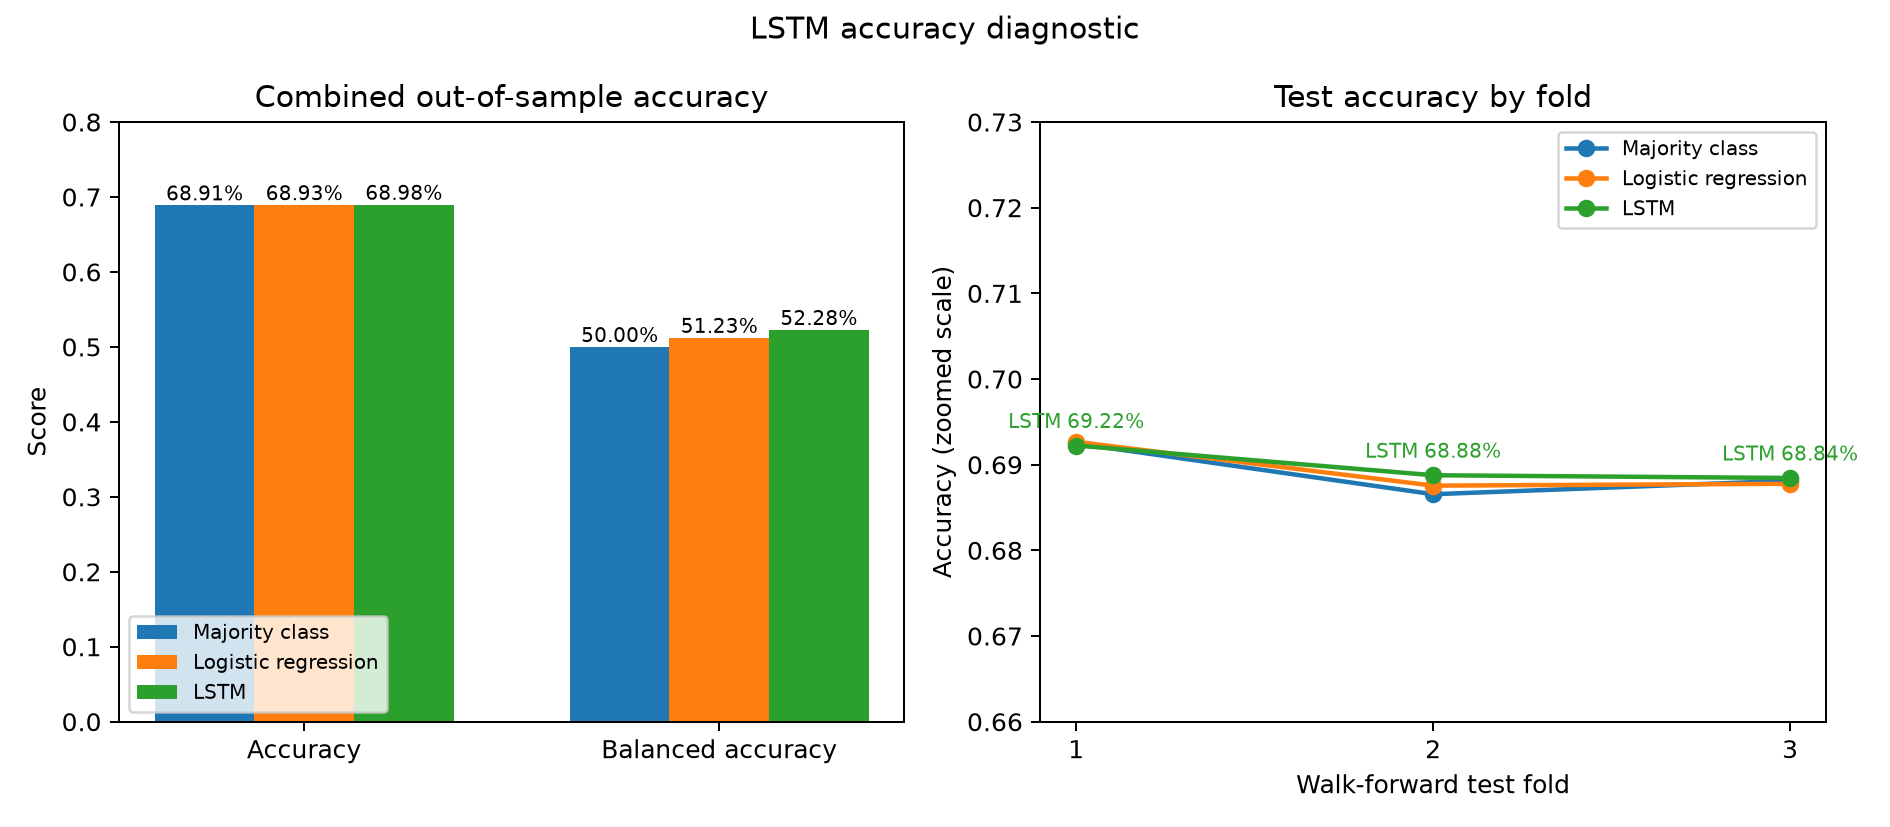
\includegraphics[width=0.98\textwidth]{qr_lstm_accuracy.png}
\caption{LSTM 准确率诊断。左图比较合并样本外 Accuracy 与 Balanced Accuracy；右图比较 3-fold 测试 Accuracy。由于类别不平衡，总体 Accuracy 必须与多数类基线、平衡准确率和排序指标一起解释。}
\label{fig:lstm-accuracy}
\end{figure}

结合上涨召回率 8.10\%、ROC AUC 0.6465 和 PR AUC 0.4276，可以得到更完整的结论：LSTM 的概率排序优于逻辑回归，但在 0.5 阈值下仍漏掉了大量上涨分钟。模型目前适合被描述为具有一定样本外排序信息，而不是已经形成高准确率或可直接交易的分钟策略。

\begin{figure}[H]\centering
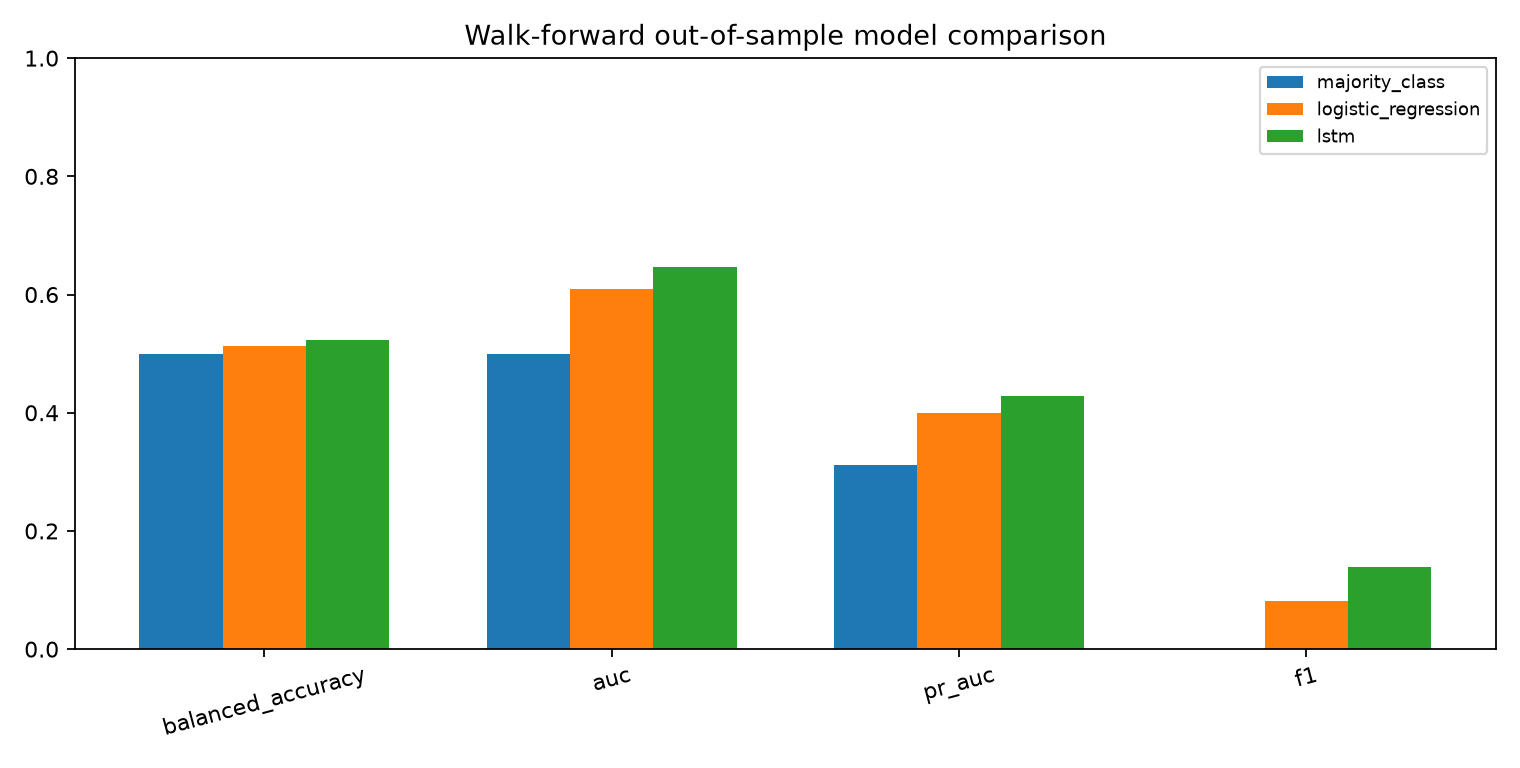
\includegraphics[width=0.88\textwidth]{qr_lstm_models.png}
\caption{多数类、逻辑回归和 LSTM 的样本外指标比较。LSTM 的排序指标高于逻辑回归。}
\end{figure}

\begin{figure}[H]\centering
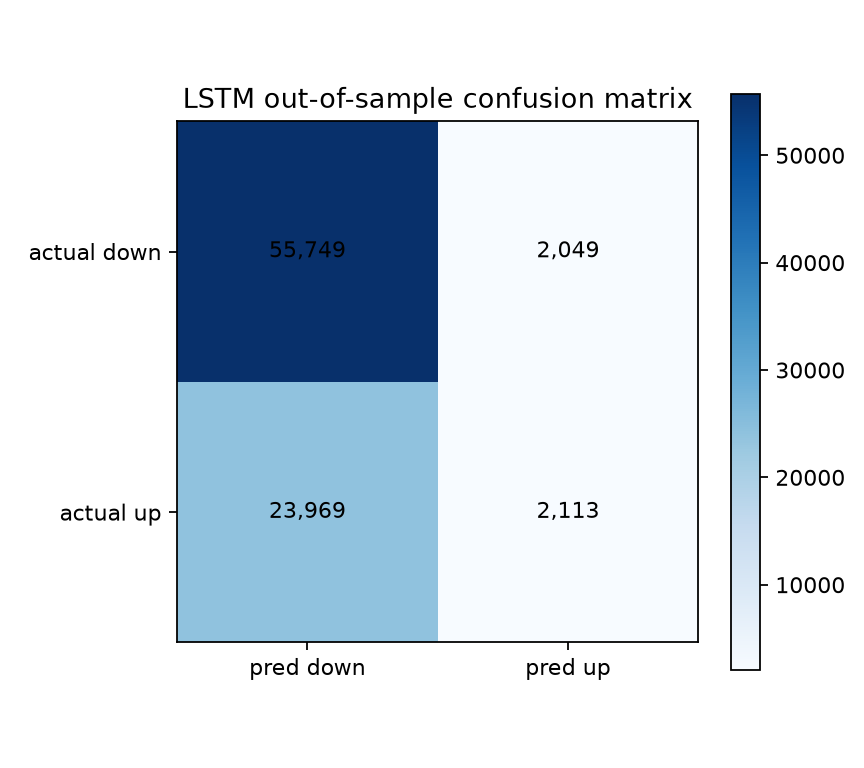
\includegraphics[width=0.72\textwidth]{qr_lstm_confusion.png}
\caption{LSTM 样本外混淆矩阵。True Positive为 2,113，False Negative为 23,969，说明 0.5 阈值下上涨召回率偏低。}
\end{figure}

\begin{figure}[H]\centering
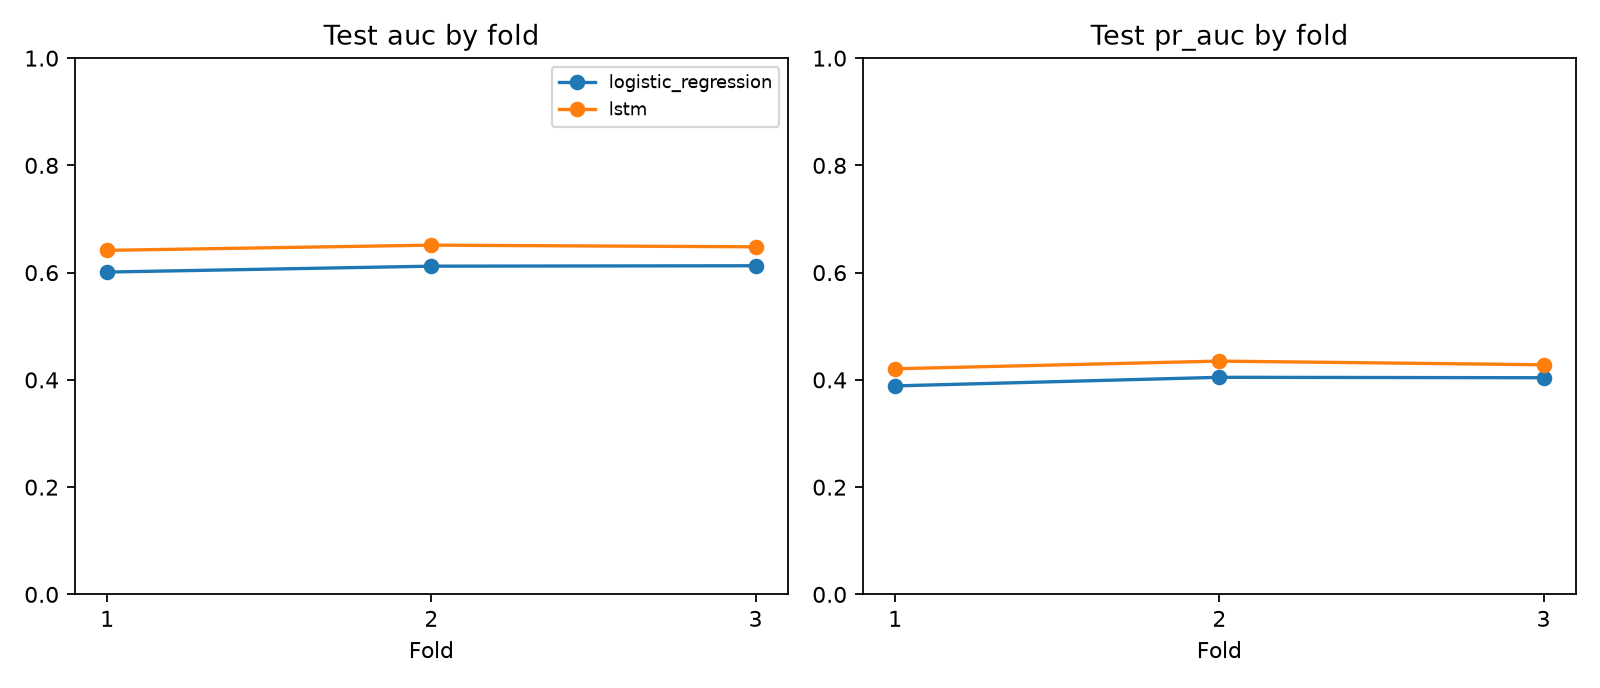
\includegraphics[width=0.92\textwidth]{qr_lstm_folds.png}
\caption{3-fold walk-forward 的逐折指标。逐折结果可用于判断表现是否集中在某一时间窗口。}
\end{figure}

LSTM 的 ROC AUC、PR AUC 和 F1 均高于逻辑回归，说明序列结构提供了一定额外排序信息；但总体准确率几乎等于多数类基线，且上涨召回率仅 8.10\%。

\chapter{结论}

\begin{itemize}
  \item 本项目共评价 18 个日频因子；新增下行波动率和特质波动率具有较强单因子结果，但与已有波动率信息高度相关，不能无条件叠加。
  \item Historical IC 加权避免了同日未来收益泄漏；Top30、每 5 日调仓和 Top60 缓冲把最新次日开盘基线的日均单边换手控制在约 8.81\%。
  \item 最终采用保留原 15 因子信号的 15\% 波动率目标。完整样本累计收益为 27.52\%，年化收益为 24.95\%，年化波动率为 16.33\%，最大回撤为 -9.58\%。
  \item 完整替换为新增风险因子、60 日 EWMA ICIR 与逆波动权重的版本未通过后 20\% 检查，因此不采用。
  \item 后 20\% 区间已参与本轮版本选择，只能作为准样本外检查；下一步需要用全新的时间区间做严格 walk-forward 验证。
  \item LSTM 的样本外排序指标高于逻辑回归，但 0.5 阈值下上涨召回率较低。
\end{itemize}

\end{CJK*}
\end{document}
